\documentclass[12pt]{support/thcolognethesis} 

\usepackage{amssymb}

\title{Optimierung von Augmented Reality Anwendungen durch die Berücksichtigung von Tiefeninformationen mit Googles Project Tango}

\degree{Masterthesis}

\author{Steffen Tröster}

\college{
	Technischen Hochschule Köln\\
    Ingenieurwissenschaftliches Zentrum\\
    Fakultät für Informations-,\\
    Medien- und Elektrotechnik}

\course{Technische Informatik (Master)}

\company{inovex GmbH}  

\firstExaminer{Prof. Dr. Hubert Randerath}
\firstExaminerLocation{Technische Hochschule Köln}
\secondExaminer{Prof. Dr. Martin Eisemann}
\secondExaminerLocation{Technische Hochschule Köln}

\degreedate{Köln, im \monthyeardate\today}
	
\begin{document}

\baselineskip=18pt plus1pt

\setcounter{secnumdepth}{3}
\setcounter{tocdepth}{3}

\maketitle                 

\begin{abstract}
\setlength{\parskip}{1em}

Project Tango ist eine neue mobile Plattform des Google Advanced Technology and Project (ATAP) Teams, die in der Lage ist, Bewegungsverfolgung, Tiefenwahrnehmung und Umgebungswiedererkennung auf Smartphones und Tablets anbieten zu können. Durch die kontinuierliche Bestimmung der relativen Geräteposition eignet sich die Plattform besonders für dreidimensionale Augmented Reality (AR) Anwendungen. Die Illusion dieser AR Anwendungen wird besonders dann gestört, wenn sich reale Objekte in einer Szene räumlich vor virtuellen Objekten befindet und diese virtuellen Objekte nicht entsprechend ausgespart werden. 

Diese Arbeit stellt daher drei Überdeckungsverfahren vor, mit denen diese Überlagerung der virtuellen Objekte mit Hilfe der Tiefenwahrnehmung von Project Tango und des Z-Buffer Algorithmus realisiert werden kann. Die Tiefeninformationen für den Z-Buffer werden hierfür zum einen direkt aus den Sensordaten und alternativ mit einer TSDF Rekonstruktion und einer selbst zusammengestellten Ebenen Rekonstruktion bestimmt. Außerdem wird auf einen zusätzlichen Ansatz eingegangen, der zur Verbesserung dieser Tiefeninformationen die Bildinformationen der Farbkamera durch den Guided Filter berücksichtigt. Diese Mechanismen werden im Laufe der Arbeit prototypisch umgesetzt und gegenübergestellt. 

\setlength{\parskip}{0em}
\end{abstract}
\selectlanguage{english}
\begin{abstract}
\setlength{\parskip}{1em}

Project Tango is a new mobile platform by Google’s Advanced Technology and Projects (ATAP) Teams, which brings Motion Tracking, Depth Perception, and Area Learning to mobile devices. With Project Tango, Google is providing a technology to tablets and smartphones for building virtual reality (VR), indoor navigation, precise measurement and augmented reality applications. The focus of this document lies mainly upon augmented reality applications. Although you can build an effective 3D AR illusion with the continuous device motion tracking, there is still a problem, that the scenes virtual object cannot be occluded by real objects when they are in foreground.

Since the Project Tango platform is offering a continues depth perception of the current viewport, this depth information can be used to solve the missing occlusion issue. This work is introducing three approaches to enable an augmented reality occlusion by real objects. Additionally an approach will be discussed to optimize the depth occlusion by taking the color information by the device’s camera into account. These methods will also get implemented with the development kit, tested, compared and evaluated concerning their applicability.

\setlength{\parskip}{0em}
\end{abstract}
\selectlanguage{ngerman}


         

\begin{romanpages}         
\tableofcontents            
\end{romanpages}          

% Einleitung
\chapter{Einleitung}

Project Tango ist eine neue mobile Plattform des Google Advanced Technology and Projects (ATAP) Teams, welche Bewegungsverfolgung, Tiefenwahrnehmung und Umgebungswiedererkennung auf mobilen Endgeräten realisiert.

\begin{quotation}
\enquote{Project Tango combines 3D motion tracking with depth sensing to give your mobile device the ability to know where it is and how it moves through space.}  \citep{Proje19:online}
\end{quotation}

Diese Verfügbarkeit dieser Echtzeitdaten ermöglicht viele verschiedene neue Einsatzmöglichkeiten auf mobilen Endgeräten wie Smartphones und Tablets. Typische Einsatzszenarien dieser Plattform sind die Indoor Navigation, die Vermessung der Umgebung sowie andere Anwendungen im Bereich Virtual und Augmented Reality. Der Fokus dieser Forschungsarbeit liegt hier in dem Anwendungsbereich der dreidimensionalen Augmented Reality (AR). 

Die Anwendungsgebiete für Augmented Reality (dt. Erweiterte Realität) sind sehr vielseitig und liegen in der Medizin, der Unterhaltungsindustrie, Bildung und in vielen weiteren Industriezweigen. Eine barrierefreie Navigationshilfe, Einblendungen für die persönliche Assistenz, kontextsensitive Projektionen und Computerspiele sind Beispiele für typische Anwendungen, die durch AR umgesetzt werden können. 

Für die erfolgreiche Umsetzen einer Augmented Reality Anwendung, müssen die Kameraeigenschaften, wie Brennweite, Verzerrung und die Position der Kamera zu jeder Zeit und idealerweise in Echtzeit bekannt sein. Sensoren wie Kompass, INS (Trägheits\-navigations\-system) oder GPS können zwar eine grobe Lokalisierung ohne bekannte Merkmale im Raum ermöglichen, führen aber langfristig zu Fehlern, wenn keine optischen Referenzen gegeben sind. Mit Hilfe von der Bewegungsverfolgung durch Project Tango kann diese Lokalisierung der Kamera und somit die korrekte Positionierung von virtuellen Objekten im Raum deutlich zuverlässiger, in Echtzeit und ohne vordefinierte Merkmale im Raum realisiert werden. Project Tango eignet sich daher sehr gut für die Umsetzung und den Einsatz von AR Anwendungen.

\section{Augmented Reality Optimierung}

Um eine für den Betrachter effektive und optimierte Augmented Reality Anwendung umsetzen zu können, benötigt man laut \citet{azuma2001recent} die Möglichkeit mehr Informationen über relevante Objekte im realen Raum ermitteln zu können. Durch diese Informationen könnte dem Nutzer zum Beispiel eine Interaktion mit realen Objekten ermöglicht werden oder anhand optischer und semantischer Einordnung der Umgebung passende Funktionen angeboten werden. 

Hinsichtlich der zuletzt erwähnten Kontextsensitivität existieren viele Ansätze, basierend auf optischen Merkmalen der Umgebung. So kann zum Beispiel ein optisches Tracking von realen Objekten, wie von \citet{lee2008hybrid} beschrieben, umgesetzt werden. Project Tango nutzt bereits optische Merkmale, um eine Positionsverfolgung oder das Lernen der Umgebung umzusetzen. Wären diese Merkmale für den Entwickler als Schnittstelle verfügbar, könnte man mit diesen Informationen solche kontextsensitiven Anwendungen umsetzen. Der Fokus soll in dieser Arbeit jedoch nicht auf den optischen Merkmalen sondern auf den Tiefeninformationen, die Project Tango durch den eingebauten Tiefensensor in Form einer Pointcloud liefern kann, liegen.

Ein sinnvoller Einsatz von Augmented Reality Anwendungen besteht darin, virtuelle Objekte in eine echte Szene zu projizieren. Dabei überlagert die Projektion des virtuellen Objekts das aktuelle Kamerabild oder den aktuellen Sichtbereich und erwirkt dadurch den Anschein, als ob sich das virtuelle Objekt wirklich in der Szene befindet. Dieser Effekt funktioniert solange erfolgreich, bis ein reales Objekt sich räumlich vor das virtuelle Objekt bewegt und die zu erwartende Überlagerung des virtuellen Objekts nicht erfolgt. Diese fehlerhafte Darstellung durch eine fehlende Überdeckung ist in Abbildung \ref{fig:occlusion-problem} zu erkennen. 

\begin{figure}[h]
  \centering
	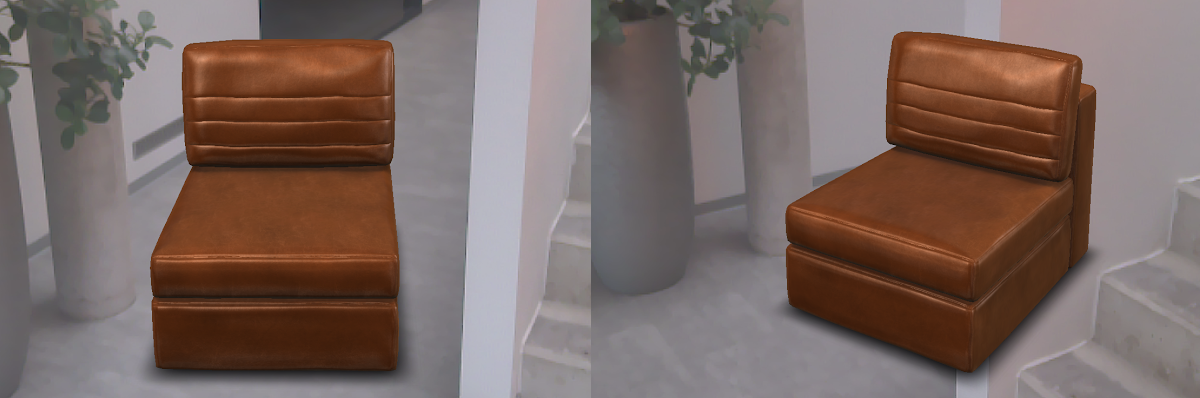
\includegraphics[width=1.0\textwidth]{content/images/occlusion-problem.png} 

  \caption{AR Projektion mit Project Tango - Links: Erfolgreiche Projektion. Rechts: Fehlerhafte Darstellung ohne Überdeckung.}
  \label{fig:occlusion-problem}
\end{figure}

Die Verfügbarkeit der Tiefeninformationen bei Project Tango könnte die Interaktionen oder Darstellungen in einer Augmented Reality Anwendung präziser an die echten räumlichen Gegebenheiten anpassen. Es existieren zum Beispiel prototypische Anwendungen, in denen virtuelle Markierungen passend an echten Objekten im virtuellen Raum positioniert werden können, indem sie auf die aktuellen Tiefeninformation des Sichtbereichs zurückgreifen. Eine weitere Idee ist es, Überlagerungen virtueller Objekte ermitteln zu können, an denen sich reale Objekte im Vordergrund befinden.

\section{Zielsetzung und Vorgehen}

Diese Arbeit will die Fragestellung beantworten, durch welche Verfahren mithilfe der Tiefeninformationen von Project Tango, automatisch und in Echtzeit die Überdeckung virtueller Objekte mit realen Objekten in einer Augmented Reality Szene realisiert werden kann. Dabei soll Project Tango als autonomes System betrachtet werden, welches diese Problemstellung selbstständig und mit den eingeschränkten Ressourcen dieser mobilen Plattform lösen soll.

Hierzu sollen zunächst bestehende Verfahren zur Bestimmung einer Augmented Reality Überdeckung durch eine Literaturrecherche gefunden werden. Diese Verfahren sollen dabei auf Ihre Anwendbarkeit mit der Project Tango Hardware überprüft werden. Sollten sich aus der Recherche weitere Ideen ergeben, wie speziell auf der Project Tango Hardware eine Überdeckung umgesetzt oder verbessert werden kann, sollen diese mit in die Arbeit eingebunden werden. Eine Idee könnte zum Beispiel sein, auch das Farbbild der normalen Kamera von Project Tango in die Optimierung der virtuellen Überlagerung einfließen zu lassen. Die identifizierten Verfahren sollen hiernach entsprechend implementiert werden, um sie darauf folgend in einer Testumgebung gegenüber zu stellen.

Strukturell wird in dieser Arbeit in Kapitel \ref{sec:thema} erst einmal auf die thematischen Grundlagen zu Augmented Reality und Project Tango eingegangen. Hier werden auch die existierenden Verfahren zur AR Überdeckung angesprochen. Unter Kapitel \ref{sec:algorithms} sind theoretische Grundlagen zu finden, die bei der späteren Umsetzung verschiedener Verfahren angewendet werden. Kapitel \ref{sec:optimization} beinhaltet die Argumentation und Beschreibung der gewählten Verfahren, welche unter Kapitel \ref{sec:implementation} auf der Project Tango Hardware umgesetzt werden. In Kapitel \ref{sec:evaluation} werden die vorliegenden Umsetzung in einem Testszenario gegenübergestellt, um eine Aussage treffen zu können, welcher Ansatz auf der Hardware oder für einen bestimmten Einsatz gut funktionieren könnte.




% Thematische Vorbemerkung
\chapter{Thematische Vorbemerkung}

Im ersten Teil dieses Kapitels werden zunächst einmal die Grundlagen zu Augmented Reality beschrieben, wie diese Technologie einzuordnen ist, welche technischen Anforderungen ein Augmented Reality System hat und wo typische Einsatzszenarien liegen. Außerdem wird hier auf den aktuellen Stand der Forschung bezüglich der Bestimmung von Überdeckungen in einem Augmented Reality System eingegangen. Hiernach wird näher auf Googles Project Tango eingegangen, welche Konzepte angewendet werden und wie diese Technologie im Bereich Augmented Reality einzuordnen ist. \\


\section{Augmented Reality}

Augmented Reality (AR) ist eine Klasse aus dem Realitäts-Virtualitäts-Kontinuum von \cite{milgram1995augmented}, welches in Abbildung \ref{fig:virtual-continuum} abgebildet ist. Diese Klasse beschreibt die Darstellungen von realen und virtuellen Informationen in einer Repräsentationsform, wobei hier reale und virtuelle Objekte in einer realen Umgebung kombiniert dargestellt werden können. Diese virtuellen Objekte sind in der realen Umgebung idealerweise fest lokalisiert und fügen sich somit in das reale Erscheinungsbild ein. Typischerweise sind AR Anwendungen interaktiv, und stellen die virtuellen Objekte in Echtzeit und dreidimensional in der realen Welt dar. Für die Definition von AR Anwendungen gibt es zudem keine Limitierung für die Darstellungstechnologie, wie zum Beispiel das Project Tango Tablett oder einem Head-Mounted-Display. AR beschränkt sich zudem nicht auf den angesprochenen Sinn - so sind zum Beispiel AR Anwendungen mit visueller, taktiler oder sogar olfaktorischer Umsetzung möglich.\\

\begin{figure}
  \centering
	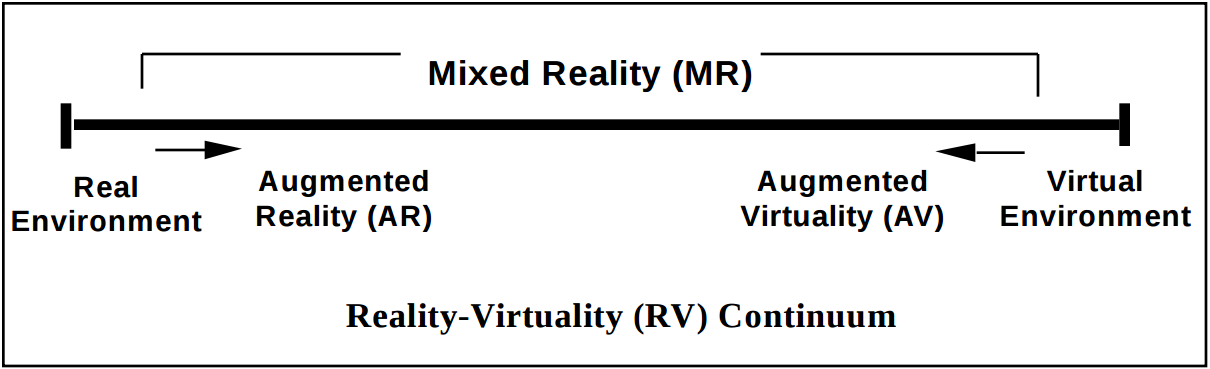
\includegraphics[width=0.85\textwidth]{content/images/theory/virtual-continuum.png} 
  \caption{Vereinfachte Darstellung des Realitäts-Virtualitäts-Kontinuum von \citet*{milgram1995augmented}}
  \label{fig:virtual-continuum}
\end{figure}


Virtuel Reality (VR) oder auch Virtual Environment hingegen kapselt sich von der realen Umgebung ab und bietet Interaktionen in reinen virtuellen Umgebungen. Diese rein virtuelle Darstellung konnte sich im Gegensatz zu Augmented Reality deutlich schneller Entwickeln, da die technologischen Anforderungen an AR deutlich höher sind. \citep{van2010survey}\\

\subsection{Technische Anforderungen}

Dieser Abschnitt widmet sich den technischen Anforderungen an Augmented Reality, indem die potentiellen Display Technologien beschrieben werden, mögliche Trackingverfahren zur Ermittlung der Betrachtungsposition erläutern werden und auch die Systeme behandelt werden, mit denen ein Nutzer mit den virtuellen Darstellungen interagieren kann.\\

\subsubsection{Display Technologie}

Der erste wichtige Teil der technologischen Anforderungen an AR sind visuelle Anzeigen (visual displays), die neben der Möglichkeit eines dreidimensionalen Renderings, welches hier aus der Virtual Reality vorausgesetzt werden soll, weitere Charakteristika mit sich bringen. Nach \citet{van2010survey} lassen sich diese Technologien zunächst in je drei Arten der Darstellung und Positionierung unterteilen.\\

Die einfachste und günstigste Art der visuellen Darstellung in AR ist \enquote{video see-through}, wodurch die reale Umgebung durch eine Video Aufnahme ersetzt wird und die virtuellen Objekte digital in die Video Aufnahme gerendert werden. Das bietet die Möglichkeit Objekte aus der realen Umgebung zu entfernen oder zu ändern oder, anhand der Luminanz Information vom Video, das Rendering der virtuellen Objekte entsprechend an die Realität anzupassen. Anwendung findet diese Technologie typischerweise in Tablets, Smartphones oder Head-Mounted-Displays.\\

Die nächste Möglichkeit zur Darstellung ist \enquote{optical see-through}. Hier werden die virtuellen Objekte durch transparente Spiegel in das Sichtfeld des Betrachters gebracht. Anders als bei \enquote{video see-throught} bleibt die reale Auflösung für die visuelle Aufnahme des Betrachtes gleich und es können zudem nur Latenzprobleme bei dem Rendering der virtuellen Objekte und nicht bei der Darstellung der realen Umgebung auftreten. Auf der anderen Seite besteht bei dieser Technologie das Problem, dass die Darstellung von virtuellen Objekten nicht kräftig genug ist, um die reale Umgebung auf Grund von der transparenten Darstellungsoberfläche komplett auszublenden. Typische Geräte dieser Technologie sind Headmounted Displays wie Google Glass\footnote{\url{https://developers.google.com/glass/} (23.02.2016)} oder stationäre Geräte wie der HoloDesk\footnote{\url{http://research.microsoft.com/en-us/projects/holodesk/} (23.02.2016)}.\\

Die dritte Möglichkeit ist die projizierte Darstellung, in der die Augmented Reality Überlagerung auf die realen Objekte projiziert werden. Diese Darstellung ermöglicht die Abdeckung vom gesamten Sichtfeld des Betrachters, benötigt aber eine entsprechende Kalibrierung oder eine Strukturwahrnehmung bei Umgebungsänderungen.\\

Neben der Art der Darstellung können die Display Technologien laut \citet{azuma2001recent} anhand Ihrer Positionierung klassifiziert werden. Man unterscheidet zwischen am Kopf befestigten Displays (head-mounted), tragbaren Displays (hand-held) und räumlich positionierten Displays. Zu jeder dieser Displayarten gibt es wiederum unterschiedliche technische Umsetzungen mit ihren spezifischen Vor- und Nachteilen bezüglich ihrer Anwendungsszenarien.\\

\subsubsection{Tracking Technologien}

Um eine virtuelle Projektion im realen Raum auf nicht stationären Displaytechnologien zu realisieren muss die Position und gegebenenfalls relative Positionsänderung des Displays bestimmt werden, auch \enquote{augmented reality registration} genannt. Man spricht dabei üblichweise von den \enquote{six degrees of freedom (6DOF)}, der Position im Raum (x, y, z) und der Orientierung (yaw, pitch, roll). \\

Frühe Techniken für die Registrierung benötigten üblicher Weise eine speziell vorbereitete Räumlichkeit, denn sie basierten auf mechanischen, magnetischen oder Ultraschall Sensoren um die Position zu bestimmen. Diese Sensoren sind zwar immer noch im Einsatz und bilden auch den Grundstein für die AR und VR Forschung, sind aber praktisch gesehen zu komplex und aufwändig für die meisten Anwendungsfälle. \citep{van2010survey} \\

Für ein grobes Positions-Tracking, vor allem auch außerhalb von Gebäuden wird GPS genutzt. Für großräumliche Anwendung ist GPS, mit einer Varianz von 10-15 Metern und in Kombination mit einem Kompass, durchaus praktikabel. Zum Beispiel um sichtbare Flugzeuge oder Sterne visuell aufzubereiten. Innerhalb von Gebäuden basiert die grobe Positionierung laut \citet{van2010survey} oft auf verfügbaren Wifi Access Points oder RFID Markern. \citet{lamarca2005place} demonstrieren hierzu auch die Möglichkeit diese Idee für grobe Lokalisation außerhalb von Gebäuden einzusetzen.\\

Optische Tracking Verfahren basierend auf Bildverarbeitung bieten laut \citet{van2010survey} deutlich genauere Resultate als die zuvor beschriebenen Verfahren. Es gibt hier viele verschiedene sensorische Ansätze ein optisches Tracking zu realisieren. Frühe verfahren, wie die von \citet{dunston2008identification} oder \citet{narzt2006augmented}, nutzten Passmarker (fiducial marker) oder Licht emittierende LEDs in einem vordefinierten Modell, um zwischen aufgenommenen Bildern die Marker oder LEDs zu detektieren und zusammengehörige zwischen den Bildern zu finden, um daraus eine Kameratransformation zu berechnen. Neue Verfahren ohne Marker, wie das sogenannte \enquote{visual odometry} von \citet{nister2004visual}, nutzen Techniken zur Feature Detection und Matching um Referenzen und Bewegungen zwischen aufgenommenen Bildern zu bestimmen.\\

Viele kommerzielle und erfolgreiche Tracking Verfahren beruhen jedoch auf hybride Ansätze, in denen die Informationen mehrerer Sensoren kombiniert werden, um potentielle Messfehler eines Sensors oder einer Methodik auszuschließen. So werden zum Beispiel Neigungssensor, Kompass und Gyroskop mit einem optischen Verfahren kombiniert, um ein Tracking der sechs Freiheitsgrade zu optimieren. Diese Erweiterung des optischen Verfahrens wird auch \enquote{visual-inertial odometry} genannt. \citep{van2010survey}\\

\citet{azuma2001recent} erwähnt an dieser Stelle auch die Kalibrierung der Sensoren, die für ein präzises Registrieren nötig ist. So müssen zum Beispiel die Linseneigenschaften der Kamera für optisches Tracking bekannt sein, damit die Verfahren mit Krümmungen, Verzerrungen und den perspektivischen Eigenschaften umgehen können. Diese Informationen sind auch bei video see-through Displays für ein korrektes Projizieren der 3D Objekte wichtig. Zudem wird erwähnt, dass man Messfehlern oder Drifts der Position zum Beispiel mit der Zunahme von Gyroscop Informationen entgegenwirken kann, indem man Ereignisse wie einen Schritt des Nutzers einfließen lässt. \citep{azuma2001recent} \\

\subsubsection{Interaktions Technologien} \label{sec:ar-interaction}

Neben den Display und Tracking Technologien ist es notwendig dem Nutzer andere Interaktionsmöglichkeiten anzubieten, da in der Regel das klassische zweidimensionale WIMP Paradigma (Windows, Icons, Menus and Pointer) im dreidimensionalen Kontext von AR keine ausreichende Gebrauchstauglichkeit bietet. Dennoch müssen die Interaktionstechnologien in Augmented Reality die üblichen Interaktionen wie aus WIMP unterstützen. Dazu gehören zum Beispiel das Auswählen, Positionieren und Drehen von virtuellen Objekten, das Zeichnen von Pfaden oder Flugbahnen, sowie die Eingabe von Quantitativen Werten oder Texten. \citep{van2010survey} \\

Frühe Augmented Realilty Systeme nutzen einfache Trackballs, Trackpads, Touchscreens oder Gyroscopmäuse für eine zweidimensionale Interaktion mit dem System. Später wurden dreidimensionale Equivalente eingeführt, wie 3D Mäuse oder Stifte, die eine dreidimensionale Interaktion ermöglichen. Diese Greifbaren Schnittstellen werden auch TUIs genannt (Tangible User Interface) und ermöglichen eine unidirektionale Interaktion mit dem System. Zudem wurden auch TUIs mit haptischen Feedback eingeführt, wie zum Beispiel die 3D Maus PHANTOM. \citep{van2010survey} \\

Eine weitere Art der TUIs sind laut \citet{azuma2001recent} Gegenstände, mit denen der Nutzer natürlich interagieren kann und die vom System optisch erfasst werden, um die Positionsänderung der Objekte anhand von Markern oder anderen optischen Merkmalen zu bestimmen. Somit kann ein Nutzer, zum Beispiel, für die virtuelle Einrichtung eines Raums, die Möbel mit Hilfe eines echten Gegenstands im Raum verschieben. \\

Nicht taktile Systeme verwenden meist optische Aufnahmen um Gesten der Hände, des gesamten Körpers oder die Blickrichtung des Nutzers zu erkennen. Dabei werden Kameras am Körper oder im Raum verwendet. Außerdem ist es Möglich Spracherkennung in die Interaktion mit einfließen zu lassen, um eine möglichst authentische Interaktion zu bieten. Wie auch bei den Tracking Technologien existieren hierbei Hybride Systeme, die verschiedene Interaktions Technologien kombinieren. \citep{van2010survey} \\

\subsection{Anwendungsbereiche}

Über die Jahre habe Wissenschaftler immer mehr Bereiche identifiziert, die von der Anwendung von Augmented Reality profitieren können. \citet{van2010survey} nennt dazu als Erstes Einsatzgebiet die persönliche Assistenz, in der AR Systeme eingesetzt werden können, um zum Beispiel mit Hilfe von Brillen (zum Beispiel der Google Glass) Namen der sichtbaren Personen anzuzeigen, die Navigation in unbekannten Regionen einzublenden oder beim Sightseeing Kontext relevante Informationen im Sichtfeld anzuzeigen. \\

Neben der persönlichen Assistenz können auch Anwendungen in der Industrie laut \citet{van2010survey} von AR profitieren. Es lassen sich zum Beispiel virtuelle Designumgebungen umsetzten, die es ermöglichen ein Auto in Lebensgröße zu Gestalten. Auch bei der Fertigung und Konstruktion können den Arbeitern unterstützende Informationen angezeigt werden. So werden zum Beispiel zu erledigende Schweißstellen hervorgehoben oder der Plan zur Konstruktion entsprechend eingeblendet. Oder für die Instandhaltung komplexer Maschinen kann ein AR System dem Nutzer eine Art Röntgenblick Hinweise auf potentielle Schwachstellen liefern. Auch in der Rüstungsindustrie existieren Anwendungsgebiete für Augmented Reality Systeme. So können zum Beispiel Gefechte für eine Kampfausbildung besser simuliert werden. \citep{azuma2001recent} \\

Für Anwendungsbereiche in der Medizin ist ein sehr genaues Tracking der Freiheitsgrade erforderlich, da AR in der Chirurgie und Behandlung von Patienten Anwendung findet. Erstellte Röntgenbilder oder Ultraschallbilder können hierdurch, anstatt auf einem separaten Monitor, direkt auf die entsprechende Körperstelle projiziert werden, wodurch gegebenenfalls eine genauere Untersuchung oder Behandlung möglich ist. \citep{van2010survey} \\

Augmented Reality wird auch im Entertainment Sektor eingesetzt. Videoübertragungen von Sportereignissen werden heutzutage oft durch zusätzliche Informationen angereichert. So erhalten zum Beispiel American Football Spiele dynamische Spielfeld Begrenzungen. Auch die Werbeeinblendungen am Rand des Spielfelds können entsprechend dem Gebiet der Ausstrahlung ausgetauscht werden. \citep{azuma2001recent} \\

Ein weiteres Großes Anwendungsgebiet für Augmented Reality sind laut \citet{azuma2001recent} Computerspiele, in denen es möglich ist in einer beliebigen Umgebung Objekte eines Spiels im Raum zu platzieren und mit Ihnen entsprechend zu interagieren. Die natürlichere Interaktion, gegenüber herkömmlichen Spielplattformen, und die Nutzung in einer persönlichen Spielumgebung führt zu einem intensiveren Spielerlebnis. \\

In der Bildung für Schulen oder Museen ist es auch mögliche AR Systeme einzusetzen. Zur Vermittlung von geometrischen oder mathematischen Grundlagen gibt es die Möglichkeit der kollaborativen und interaktiven Visualisierung von Körpern, an denen etwa Parameter manipuliert werden, um danach Ihre Eigenschaften zu beobachten. \citep{van2010survey} \\

\subsection{Einschränkungen und Probleme}

Die frühen Augmented Reality Systeme sind auf Grund ihrer Größe sehr unhandlich und mobil daher nur mit großem Aufwand anwendbar. Durch die Verfügbarkeit mobiler und performanter Endgeräte ist ein mobiler Einsatz wiederum ermöglicht worden. Jedoch besitzen die aktuellen Geräte wie Smartphones oder Tabletts nicht die entsprechende Sensorik für ein präzises Tracking der sechs Freiheitsgrade. \citet{van2010survey} weisen zudem darauf hin, dass die Registrierung der Tiefe für die Anwendung von Überdeckungen oder korrekter Positionierung bei einer Interaktion ein komplexes Problem sei. Wie in Kapitel \ref{sec:theory_project_tango} zu finden geht Project Tango dieses Problem der Sensorik entsprechend an und Versucht Schnittstellen zu bieten, um sowohl das Tracking zu ermöglichen und Tiefeninformationen über die aktuelle Szene zu liefern. \\

Eine weitere erwähnenswerte Problematik ist neben der sensorischen Themen von Augmented Reality die Herangehensweise zur Gestaltung der Nutzeroberflächen für AR. Denn die UI Konzeption gestaltet sich, laut \citet{azuma2001recent}, als schwierig. Die Anreicherungen durch Augmented Reality führt schnell dazu, dass das Sichtfeld überladen wirkt. Jedoch sollte dem Nutzer immer die Informationen zur Verfügung gestellt werden, die gegebenenfalls kontextsensitive und relevant sind. Diese Angesprochenen Faktoren führen aktuell bei Augmented Reality Anwendungsgebieten noch zu einer geringen Akzeptanz der Endverbraucher.\\

\subsection{Realisierung von Augmented Reality Über\-deckungen}

\citet{wloka1995resolving} bilden den Grundstein für die verschiedenen existierenden Ansätze für eine Augmented Reality Überdeckung von virtuellen Objekten. Sie stellen in Ihrer Arbeit ein Verfahren vor, welches mit Bildern aus einer Stereo Kamera ein Stereomatching durchführt und dadurch ein Tiefenbild generiert. Dieses Tiefenbild führt in dem Renderingprozess mit Hilfe des Z-Buffer Algorithmus (beschrieben in Kapitel \ref{sec:z-buffer}) zum Ausschluss von Teilen der virtuellen Objekte, die von realen Objekten überlagert werden. Das Ergebnis des Stereomatchings ist in ihrer Arbeit mit gewissen Ungenauigkeiten behaftet und generiert unerwünschte Lücken in der Projektion des virtuellen Objekts. Arbeiten wie von \citet{seo2013direct}, mit neuen Tiefensensoren wie der Microsoft Kinect\footnote{Microsoft Kinect - https://dev.windows.com/en-us/kinect (04.03.16)}, erhalten durch den selben Mechanismus deutlich bessere Ergebnisse. \\

Die Arbeit von \citet{breen1996interactive} nahmen diesen Ansatz von \citet{wloka1995resolving} auf und stellten die Idee vor, neben einer deutlich genaueren Überdeckung auch eine Interaktion mit realen Objekten zu realisieren. Hierfür mussten die virtuellen Modelle an der echten Umgebung passend ausgerichtet werden, was wiederum voraussetzt, dass die entsprechenden virtuellen Modelle für die realen Objekte bereits vorliegen. Nach dieser Ausrichtung wird die Tiefe der virtuellen Objekte gewonnen, um daraus mit dem Verfahren von \citet{wloka1995resolving} eine Überlagerung zu bestimmen. \\

Neben den Modell basierten Verfahren existieren auch Kanten basierte Verfahren, wie das von \citet{berger1997resolving}, in dem Objektkanten auf optischer Basis mit Filtern ermittelt werden. Diese Kanten werden über mehrere Bilder verfolgt, um die Tiefeninformation der Kanten durch Epipolargeometrie und Heuristiken zu bestimmen. \citet{berger1997resolving} gewinnt darauf folgend  eine Tiefenmaske, indem er annimmt, dass Konturen, die unter einer gewissen Distanz von einander entfernt sind, zu einem Objekt gehören. \citet{klein2004sensor} erreichen mit einer, auf mobiler Hardware umgesetzten Umgebung, mit diesem Verfahren, sehr überzeugende Ergebnisse in einer vordefinierten Umgebung. Zwar verspricht dieses Vorgehen eine Kantengenau Überdeckung virtueller Objekte, führt aber bei komplexeren Szenen, in denen die Kanten nicht mehr erfolgreich verfolgt werden oder nicht zu einem Objekt zugeordnet werden können, zu Fehldarstellungen. Außerdem werden Ausbreitungen innerhalb des Objektes, welche nicht als Kante erkannt werden können, nicht berücksichtigt.\\

Die letzte Variante wurde von \citet{breen1996interactive} bereits erwähnt, ist die Ermittlung der Überdeckung durch eine Rekonstruktion der Szene. Dieser Ansatz verschiebt durch das Verfahren von \citet{wloka1995resolving} die Problemstellung der AR Überdeckung in den Bereich der Rekonstruktionsprobleme. Bekannte Verfahren hierfür sind zum Beispiel KiniectFusion von \citet{newcombe2011kinectfusion} oder die Echtzeit Rekonstruktion von \citep{niessner2013real}. Diese sehr komplexen Verfahren sind meist auf der Grafikhardware von Desktopsystemen umgesetzt, generieren jedoch detaillierte Rekonstruktionen, die für eine Überdeckung in Augmented Reality Systemen zu evaluieren gilt. Vorteilhaft bei einer Rekonstuktions basierter Überdeckung ist zudem, dass auch Interaktionen mit echten Objekten, wie bei \citet{breen1996interactive}, erfolgreich umgesetzt werden können.





\section{Project Tango} \label{sec:theory_project_tango}

Project Tango ist eine Technologie Plattform für Android Tablets und Smartphones von Google’s Advanced Technology and Projects Group (ATAP). Das Ziel dieser Plattform ist es Motion Tracking (Positionierung), Depth Perception (Tiefeninformation/Pointcloud) und Area Learning (Lokalisierung) auf mobile Endgeräte zu bringen, um verschiedenste Anwendungs-Szenarien abzudecken. Typische Szenarien sind Indoor Navigation, Virtual Reality Anwendungen, Vermessungs- und Rekonstruktions Software und Augmented Reality Anwendungen.\\

Das System ermöglicht in erster Linie ein Tracking von Positionsänderungen des Geräts im Raum und bietet somit eine genaue relative Lokalisierung. Mit Hilfe dieser Lokalisierung und der Hinzunahme von visuellen Merkmalen im Raum, ist das Gerät in der Lage, seine Umgebung kennenzulernen und gegebenenfalls die Lokalisierung zu korrigieren oder aber Diese in einer bereits erlernten Umgebung zu ermitteln. Zusätzlich bietet Project Tango die Möglichkeit mit Hilfe eines Tiefensensors eine Pointcloud der Tiefeninformation pro Bildausschnitt zu ermitteln, um Anwendungen auch Räumliche Informationen bereitzustellen.  \citep{Proje19:online} \\

\subsection{Geräte und Hardware}

Da das Project Tango zum Zeitpunkt der Verfassung dieser Thesis noch unter Entwicklung steht, gibt es von Google die Entwickler Prototypen. Das Erste Gerät im Smartphone Format, welches in Abbildung \ref{fig:tango-device} rechts unten zu erkennen ist, wurde bereits durch eine neue Generation rechts oben ersetzt. Dieses 7\dq Tablet verfügt, wie in Abbildung \ref{fig:tango-device} links zu erkennen, über einen Infrarot Laser Projektor, eine Fisheye Camera und eine normale 4 Megapixel Kamera auf der Rückseite. Zudem sind, wie in aktuellen Smartphones und Tables üblich, ein Beschleunigungssensor, Umgebungslichtsensor, Barometer, Kompass, GPS und ein Gyroskop verbaut. Das Gerät wird von einem NVIDIA Tegra K1 Prozessor betrieben und verfügt über 4GB Arbeitsspeicher. \citep{Proje19:online} Mit diesem Gerät wurden die später beschriebenen Techniken umgesetzt und evaluiert. \\

\begin{figure}[h]
  \centering
	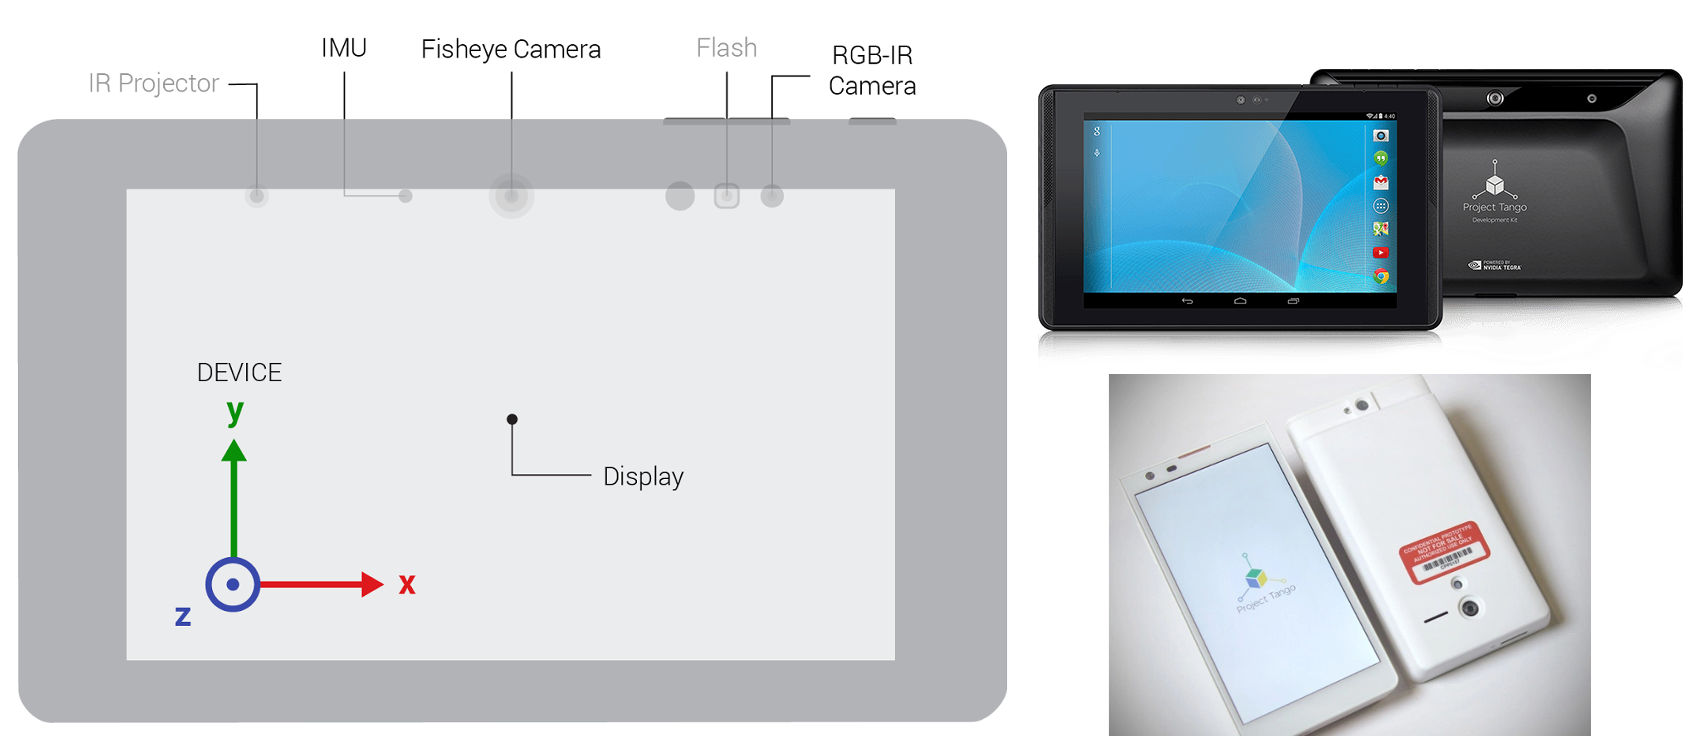
\includegraphics[width=1.0\textwidth]{content/images/theory/tango-device.png} 
  \caption{Links: schematischer Aufbau der Google Project Tango Hardware. Rechts: Das aktuelle Entwickler Gerät im Tablet Format (oben) und das alte Entwickler Gerät im Smartphone Format (unten). Übernommen von \citet{GoogleDevelopers:online}}
  \label{fig:tango-device}
\end{figure}

\subsection{Konzepte und Schnittstellen}

Generell betrachtet ist das Project Tango eine Plattform, die Computer Vision nutzt, um dem Gerät die Möglichkeit bietet seine relative Positionierung in der umgebenen Szene live zu bestimmen. Auf den Geräten kommt Googles Android zum Einsatz, weshalb zu beachten ist, dass es sich bei der Platform nur bedingt um eine Echtzeit Umgebung handelt. Das liegt daran, dass der Linux Kernel keine Garantien für die zeitlich präzise Ausführung von Instruktionen auf Grund von Scheduling geben kann. Google weist daher darauf hin, dass das System als \enquote{soft-realtime} betrachtet werden sollte. Daher sollten Messergebnisse verschiedener Sensoren unter Berücksichtigung ihrer Aufnahme Zeitpunkte verwendet werden. \citep{GoogleDevelopersConcepts:online} \\

\subsubsection{Motion Tracking}

Um die relative Bewegung vom Start des Project Tango Systems bestimmen zu können nutzt es \enquote{visual-inertial odometry}. \citep{GoogleDevelopersConcepts:online}
Dabei handelt es sich um eine erweiterte Variante von Visual Odometry. 
Das von \citet{nister2004visual} veröffentlichte Verfahren Visual Odometry ist in der Lage aus einfachen Video Inhalten in Echtzeit die Bewegung der Kamera zu bestimmen. 
Hierzu werden zunächst übergreifende Features, zum Beispiel Punkte aus der \citet{harris1988combined} Kantenerkennung, aus mehreren Bildern bestimmt. Um nun eine Transformation zwischen den Bildern ermitteln zu können wird der 5-point Algorithmus von \citet{nister2004efficient} angewendet. Dieser Algorithmus ist in der Lage das Problem zu lösen, eine relative Transformation zwischen zwei Bildern mit gegebenen 5 Punktübereinstimmungen zu ermitteln. Außerdem wird erwähnt, dass mit Hilfe des Schätzverfahrens RANSAC (beschrieben in Absatz \ref{sec:ransac}) bei einer Überbestimmung des Modells, ein potentieller Fehler deutlich minimiert werden kann. \\

Project Tango lässt an dieser Stelle die internen Sensoren zur Rotation, Orientierung und Bewegung mit in die Bestimmung der Kamera Transformation einfließen, um so ein akkurates Ergebnis erzielen zu können. Über eine längere Messzeit oder eine größere Entfernung vom Ursprung kann es jedoch zu kleinen Abweichungen kommen. Außerdem existiert zum aktullen Zeitpunkt noch ein \enquote{drift} Problem, was zu großen Messfehlern führen kann. Es wird jedoch versucht diese Probleme mit dem Konzept \enquote{Area Learning}, beschrieben in Kapitel \ref{subsec:area-learning}, zu lösen. \citep{GoogleDevelopersConcepts:online}
Wie genau das Verfahren aussieht, welche Techniken zur Feature Detection oder Feature Matching genutzt wird und welche Features hierfür erkannt werden ist nicht bekannt. \citet{Klingensmith_2015_7924}, als Mitglieder Googles Advanced Technologies and Projects Abteilung ATAP, erwähnen jedoch, dass nähere Informationen über das Verfahren von \citet{kottas2013consistency} und \citet{mourikis2007multi} verfasst wurden. \\

\subsubsection{Deph Perception}

Zur Tiefenmessung ist die Project Tango Hardware mit einem kalibrierten Infrarot Laser Projektor ausgestattet. Dieser streut Infrarot Punkte mit einer Auflösung von 320 x 180 Punkten in den Raum, um dann, mit Hilfe von Aufnahmen der RGB Kamera, eine Punktewolke der Tiefeninformation zu bestimmen. Auf Grund einer ausgewogenen Konfiguration zwischen Messbereich, Messfehlern und dem Energieverbrauch, liegt der Messbereich der Sensorkombination, laut \citet{GoogleDevelopersConcepts:online}, zwischen einem halben und vier Metern. \\

Dadurch dass diese Technologie auf der Aufnahme von projiziertem Infrarot Licht basiert, ist ein Einsatz der Tiefenmessung außerhalb geschlossener Räume nicht möglich. \citep{GoogleDevelopersConcepts:online} Außerdem entstehen Messfehler durch reflektierende,  lichtabsorbierende oder zu komplex strukturierte Oberflächen, wie zum Beispiel Metalle, LCD Monitore oder Hochflor Teppiche. \\

Die zuvor erwähnten Punktewolken werden in dem eigens definierten XYZij Format von der Entwicklungsschnittstelle zurück gegeben. Dabei wird jeder Punkt mit den \(X\),\(Y\) und \(Z\) Koordinaten und den beiden Indizes \(i \) und \(j \) für die Spalte und Zeile der projizierten Punkte auf die Bildebene angegeben. \citep{GoogleDevelopersConcepts:online} Man spricht dabei von einer organisierten Punktewolke, da durch die \(i\) und \(j\) Koordinaten die direkten Nachbarn, ausgehend von dem Aufnahmeblickwinkel, eines Punktes bestimmt werden können. Hieraus ist es möglich Tiefenbilder, die sogenannten \enquote{Depth Maps}, zu bestimmen, für die es viele verschiedene Computer Vision Verfahren zur Bestimmung von Objekten, Strukturen und Fluchtpunkten gibt. Die Ermittlung der Spalten \(i\) und Zeilen \(j\) sind jedoch laut \citet{GoogleDevelopersKnownIssues:online} noch nicht in den Schnittstellen enthalten.\\ 

\citet{GoogleDevelopersConcepts:online} weist darauf hin, dass das Generieren von Polygon basierten Rekonstruktionen noch nicht in den Schnittstellen enthalten sind. Es gibt jedoch freie Dritt-Bibliotheken und -Systeme, wie das Robot Operating System \citep{ROS} oder die Point Cloud Library \citep{pcl}, die für eine weitere Verarbeitung genutzt werden können.

\subsubsection{Area Learning} \label{subsec:area-learning}

Area Learning bezeichnet den Prozess indem Project Tango Geräte in der Lage sind durch visuelle Hinweise die umgebenen Welt kennenzulernen und auf die Position des Gerätes zu schließen. 
Es ermöglicht somit eine Unterstützung für Motion Tracking und löst das Problem das Gerät in einer bereits bekannten Umgebung zu lokalisieren, wie in Abbildung \ref{fig:area-learning} links zu erkennen.
Project Tango bietet außerdem die Möglichkeit diese visuellen Hinweise und Ihre Position im Raum in sogenannten \enquote{Area Description Files} zu speichern und wiederzuverwenden. \citep{GoogleDevelopersConcepts:online}\\

\begin{figure}[h]
  \centering
	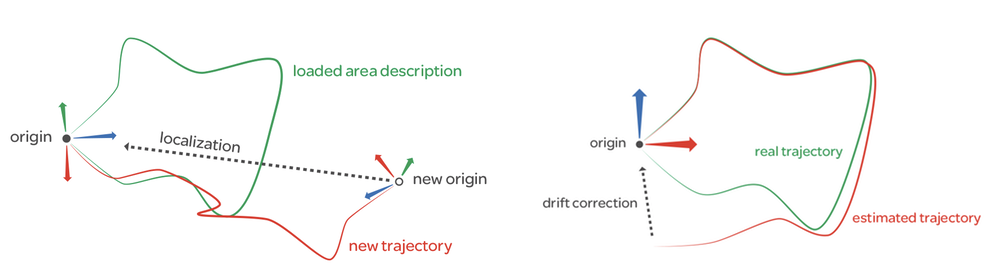
\includegraphics[width=1.0\textwidth]{content/images/theory/tango-area-learning.png} 
  \caption{Links: Lokalisierungsprozess durch Area Learning. Rechts: Korrigierung von Motion Tracking anhand gelernter Merkmale . Übernommen von \citet{GoogleDevelopers:online}}
  \label{fig:area-learning}
\end{figure}

Wie bereits erwähnt entstehen bei Motion Tracking über eine längere Strecke Messfehler. 
Während diese Strecke mit einem Project Tango Gerät abgelaufen wird, ermittelt es fortlaufend die Position und den Pfad, den der Nutzer im Raum gegangen ist. 
Erkennt es während der Strecke visuelle Merkmale aus Area Learning, wird der Pfad anhand der Positionen der Merkmale entsprechend angepasst. 
Project Tango unterscheidet hier zwischen zwei Manipulationen, \enquote{loop closures}, zur Zusammenführung des Pfads wenn ein Kreis gelaufen wurde, und \enquote{drift corrections}, um den erwähnten drift Effekt bei zu wenigen optischen Features im visual-inertial odometry. 
Die drift correction ist in Abbildung \ref{fig:area-learning} rechts zu erkennen. \citep{GoogleDevelopersConcepts:online} \\

Auch bei diesem Prozess werden die genauen Details nicht näher erläutert und es ist nicht bekannt wie die area desciptions definiert sind oder was sie enthalten. \citep{GoogleDevelopersConcepts:online} weist jedoch darauf hin, dass auch wenn die Area Desciptions Files keine direkten Bilder enthalten, es möglich sei, Rückschlüsse auf die gelernte Umgebung ziehen zu können. \\

\subsection{Einordnung zu Augmented Reality} \label{sec:classification_project_tango}

Da sowohl die Grundlagen aus dem Bereich Augmented Reality und die technische Basis von Project Tango bekannt ist, kann die Project Tango Hardware bezüglich Augmented Reality näher eingeordnet werden. Bei der Hardware handelt es sich um ein hand-held Gerät, welches mit einer video see-through Display Technologie Augmented Reality Anwendungen ermöglicht. Hierfür kann wahlweise die normale RGB Kamera oder die Graustufen Fish-Eye Kamera verwendet werden. Denn für beide Kameras können die intrinsischen Kameraparameter ausgelesen werden, wodurch die Eigenschaften realen Kamera durch die virtuelle Kamera übernommen werden können. Das führt zu einer parallax freien Überblendung und zu einer guten Tiefenwahrnehmung. \\

Als Tracking Technologie wird hier eine hybride optische Variante angewendet, die Visual Odometry mit der Fish-Eye Kamera wird durch interne Sensoren für die Rotation, Orientierung und Bewegung kombiniert. Außerdem kann das Verfahren gegebenenfalls durch Googles Area Learning Mechanismen angereichert werden, um Messfehler entgegenzuwirken. \\

Die Eingabe erfolgt durch den Touchscreen des Tablets. Eine Interaktion mit Hilfe von optischer Gestenerkennung oder anhand der Tiefeninformationen ist zudem auch möglich. \\







% Theoretische Grundlagen
\chapter{Theoretische Grundlagen}

In diesem Kapitel werden die Theoretischen Grundlagen und Algorithmen näher erläutert, die zur Realisierung der Optimierungsverfahren im nachfolgenden Kapitel \ref{sec:optimization} angewendet werden. 



\section{Z-Buffer Algorithmus} \label{sec:z-buffer}

Der Z-Buffer Algorithmus, welcher fast zur selben Zeit von \citet{straber1974schnelle} und \citet{catmull1974subdivision} vorgestellt wurde, ermöglicht in der Computergrafik eine einfache Berechnung der Überdeckungen von gerenderten Objekten auf der Bildebene. Hierzu wird neben der Bildebene noch ein sogenannter \enquote{Z-Buffer} eingeführt, der für jeden gerenderten Pixel auf der Bildebene eine Tiefeninformation festhält. Initial enthält der gesamte Z-Buffer die Tiefeninformation die der Backclipping-Ebene entspricht. Somit lässt sich für jeden Pixel einer bestimmten Position bestimmen, ob dieser einen kleineren Tiefenwert besitzt und somit auf die Bildebene gerendert wird. \\

Heutzutage ist dieser leicht zu implementierende Mechanismus aus Performancegründen in nahezu jeder Grafikkarte in Hardware implementiert. Das Problem bei dieser einfachen Umsetzung ist jedoch, dass jedes Objekt der Szene gerendert werden muss, auch wenn es später auf der Bildebene nicht erscheint. Abhilfe für dieses Problem bietet der Hierarchical Z-Buffer von \citet{greene1993hierarchical}, welcher nicht sichtbare Objekte zuvor aussortiert. Für die Anwendung für die Optimierungsverfahren in Kapitel \ref{sec:optimization} ist jedoch nur die Idee aus des einfachen Z-Buffers relevant.

\section{RANSAC} \label{sec:ransac-theory}

Der \enquote{RAndom SAmple Consensus} Algorithmus (RANSAC), vorgestellt von \citet{fischler1981random}, ist in der Lage, aus einer Menge von Daten mit vielen Ausreißern, die Parameter für ein passendes Modell zu schätzen. Anders als andere Schätzverfahren wie \enquote{Least-Median} oder \enquote{M-Schätzer}, welche aus der Statistik Literatur entnommen und entsprechend angepasst wurden, wurde RANSAC speziell für die Anwendung in der Computer Graphik entwickelt. Der Kern dieses Algorithmus ist das wiederholte Bestimmen eines Modells aus zufälligen und für das Modell ausreichenden Stichproben. Listing \ref{lst:ransac} zeigt den Verlauf des RANSAC Algorithmus. Die Anzahl der Iterationen \(N\) hängt dabei allein von dem Anteil der Ausreißer in den Messwerten ab. Daher sollte sie entsprechend gewählt werden, um die Wahrscheinlichkeit zu verringern, dass Ausreißer in den Stichproben enthalten sind. \citep{derpanis2010overview} \\

\begin{lstlisting}[mathescape,caption=Der RANSAC Algorithmus, label=lst:ransac, float=htbp]
Eingabe: Messwerte $P$, Modelltoleranz $e$, maximale Iterationen $N$
Ausgabe: Modell $m$, Unterstützende Messwerte $P_m$

1. Wähle zufällig so viele Stichproben aus den Messwerten $P$,
   wie nötig sind, um das Modell zu bestimmen
2. Bestimme aus den gewählten Stichproben das Modell $m$
3. Ermittle die Anzahl der Messwerte $P$, die mit einer 
   entsprechenden Toleranz $e$ das ermittelte Modell $m$ 
   unterstützen
4. Wenn prozentual genügend Messwerte aus $P$ das Modell $m$ 
   unterstützen dann terminiere und gehe zu 7
5. Wenn $|P_m| < |P|$ dann $|P_m| = |P|$
6. Wiederhole die Schritte 1-4 $N$ mal
7. Ermittle aus den unterstützenden Messwerten $P_m$ erneut 
   das finale Modell $m$
   
\end{lstlisting} 

Die in Schritt sieben beschriebene erneute Modellermittlung kann laut \citet{fischler1981random} durch ein ein Regressionsverfahren wie der Methode der kleinsten Quadrate bestimmt werden. Anwendung findet dieser Algorithmus in der Ebenendetektion aus Kapitel \ref{sec:ransac}.

\section{Ermittlung der konvexen Hülle}

Für die Bestimmen der konvexen Hülle von Punkten \(P\) in \( \mathbb{R}^2\) existieren verschiedenste Algorithmen, wie zum Beispiel der Monotone Chain von \citet{andrew1979another}, QuickHull nach \citet{eddy1977new} oder den Divide-and-Conquer Algorithmus von \citet{preparata1985convex}. Da alle diese Algorithmen ein ähnliches Laufzeitverhalten aufweisen, wird für die spätere Anwendung hier exemplarisch der Graham Scan nach \citet{graham1972efficient} näher erläutert. Dies ist einer der populärsten Algorithmen für die Berechnung der konvexen Hülle und besitzt eine Komplexität von \(O(n \log n)\).\\

Gestartet wird der Algorithmus mit der Menge aller Punkte \(P\) der Ebene und mit einem Startpunkt \(P_0\), der Bestandteil der konvexen Hülle ist. Hierzu wird meist der Punkt mit dem niedrigsten \(y\) Faktor gewählt. (\(P_0=P_{min(y)}\)) Listing \ref{lst:graham-scan} zeigt den Verlauf des Algorithmus des Graham Scans. Dabei wird in Abbildung \ref{fig:convexhull} nochmals die erste Sortierung und das Unterscheidungskriterium für die Sortierung als auch für die Aussortierung der Punkte verdeutlicht. \citep{convexHull} \\


\begin{lstlisting}[mathescape,caption=Graham Scan Algorithmus, label=lst:graham-scan, float=htbp]
Eingabe: Menge der Punkte $P$, außen liegender Punkt $P_0$
Ausgabe: Punkte der konvexen Hülle

$i$ = 0
sortiere nach dem Winkel zu $P_0$
solange $i$ <= $|P|$
    wenn $\measuredangle P_{i-1} P_{i}$ > $\measuredangle P_{i-1} P_{i+1}$, also $P_i$ rechts von  $\vec{P_{i-1} P_{i+1}}$ liegt
        inkrementiere $i$
    ansonsten
        entferne $P_i$ aus $P$
        dekrementiere $i$
    
\end{lstlisting} 

\begin{figure}[h]
  \centering
	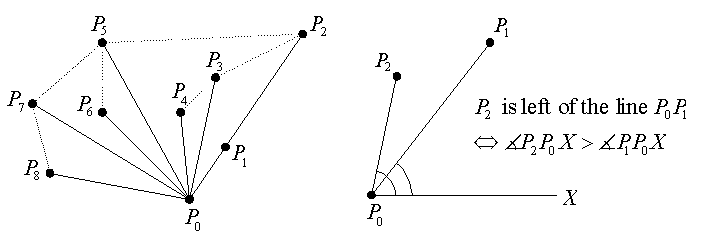
\includegraphics[width=0.9\textwidth]{content/images/methods/convexhull.png} 
  \caption{Sortierung der Punkte nach Winkel zum Startpunkt (links) mit dem Unterscheidungskriterium (rechts). Übernommen von \citet{convexHull}}
  \label{fig:convexhull}
\end{figure}


\section{Octree}

Ein Octree ist zunächst eine Datenstruktur, die wie ein Baum mit beliebiger Tiefe aufgebaut ist und pro Knoten Acht Kinder besitzt. Die Funktion ist dabei in \(\mathbb{R}^3\) gleich zu einem Binärbaum in \(\mathbb{R}\) oder einem Quadtree in \(\mathbb{R}^2\). Ein Knoten repräsentiert im Octree einen Würfel, der durch seine Kinder in Acht Kind-Würfel aufgeteilt wird. Diese Aufteilung ist in Abbildung \ref{fig:octree} exemplarisch dargestellt.\\

\begin{figure}[h]
  \centering
	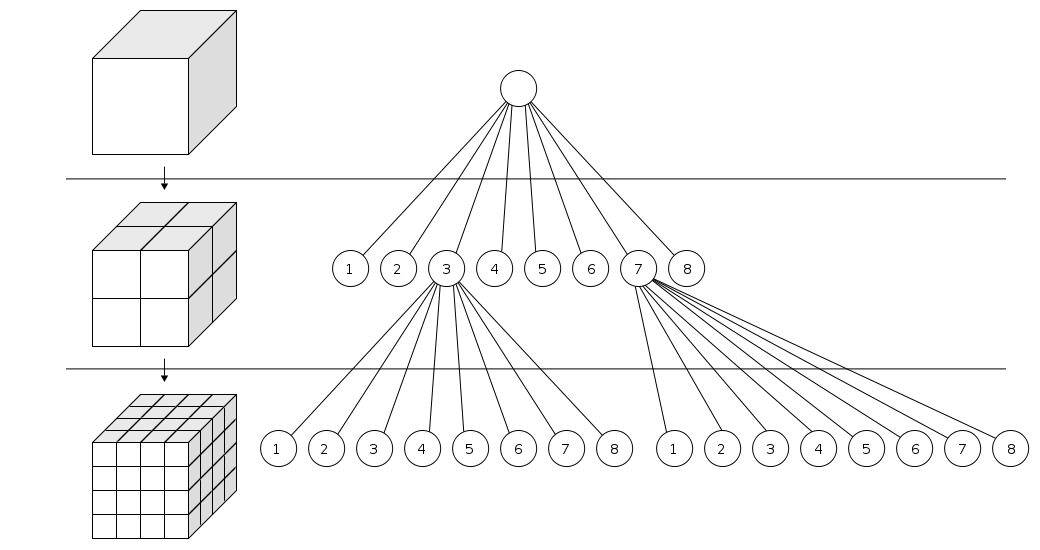
\includegraphics[width=1.0\textwidth]{content/images/theory/octree.png} 
  \caption{Schematische Darstellung eines Octrees mit zwei Untergliederungen. Übernommen von \citet{dumusc2011multi}}
  \label{fig:octree}
\end{figure}

Durch diese räumliche Aufteilung ergeben sich verschiedene Vorteile gegenüber linearen Datenstrukturen. So müssen Bereiche zum festhalten räumlicher Informationen im Octree nur dann allokiert werden, wenn diese Bereiche auch verwendet werden. Außerdem kann man mit Hilfe von Octrees ein einfaches Downsampling von Daten ermöglichen. Speichert man Punkte in den untersten Knoten eines Octrees kann man durch eine Tiefenbegrenzung beim Zugriff auf den Baum ein sehr effektives Downsampling der Punkte vornehmen. Zudem kann ein Octree zum einfachen räumlichen Clustern von dreidimensionalen Objekten dienen.\\

% Optimierung von AR
\chapter{Verfahren zur Optimierung von Augmented Reality durch Tiefeninformationen}

Anhand der Klassifizierung von Project Tango bezüglich Augmented Reality aus Abschnitt \ref{sec:classification_project_tango}, kann bereits festgehalten werden, dass sich das Gerät, durch die Verfügbarkeit von intrinsischen und extrinsischen Kameraparametern, für den Einsatz von Augmented Reality gut eignet. Um jedoch eine für den Betrachter eine effektive und optimierte Augmented Reality Anwendung umsetzen zu können, benötigt man laut \citet{azuma2001recent} die Möglichkeit mehr Informationen über relevante Objekte im realen Raum zu ermitteln. Diese Informationen könnten zum Beispiel eine Tiefenüberdeckung von virtuellen Objekten durch reale Objekte ermöglichen, eine Interaktion mit realen Objekten durch die Anwendung von physikalischen Modellen und Kollisionen generieren oder die Funktion anhand semantischer Einordnung der Umgebung variieren. \\

Zur zuletzt erwähnte Kontextsensitivität existieren viele Ansätze, basierend auf optischen Merkmalen der Umgebung. So kann zum Beispiel ein optisches Tracking von realen Objekten, wie von \citet{lee2008hybrid} beschrieben, umgesetzt werden. Project Tango nutzt bereits optische Merkmale um \enquote{Motion Tracking} und \enquote{Area Learning} umzusetzen. Wären diese Merkmale für den Nutzer als Schnittstelle verfügbar, könnte man mit Diesen solche kontextsensitiven Anwendungen umsetzen. Der Fokus soll hier jedoch nicht auf den optischen Merkmalen liegen. Die Information, auf die sich hier fokussiert werden sollen sind die Tiefeninformationen, die Project Tango durch \enquote{Depth Perception} in Form einer Pointcloud liefern kann.\\

Die folgenden Abschnitte widmen sich den Verfahren zur möglichen Realisierung dieser Optimierungen durch Tiefeninformationen. Zunächst wird beschrieben, wie eine mögliche Interaktion mit Oberflächen der realen Welt durch eine Pointcloud ermöglicht werden kann. Hiernach wird ein Verfahren beschrieben, was ermöglicht eine Überdeckung virtueller Objekte durch Depth Maps umzusetzen. Diese Idee kann, wie dort näher erläutert, weitergeführt werden, indem existierende Verfahren zur Echtzeit Rekonstruktion von Oberflächen näher behandelt werden. Außerdem wird eine Idee als Verfahren beschrieben, die im laufe dieser Arbeit entwickelt worden ist, um basierend auf verschiedensten Algorithmen eine planare Echtzeitrekonstruktion zu ermöglichen. Zuletzt soll näher auf die Möglichkeit eingegangen werden, die resultierenden Tiefeninformationen aus der Pointcloud oder aus dem Rendering der Rekonstruktion mit Hilfe der Bildaufnahmen der Farbkamera, zu verbessern. \\

Die hier beschriebenen Verfahren zur Tiefenwahrnehmung für die Anwendung in Augmented Reality werden im Laufe dieser Arbeit umgesetzt und gegenübergestellt. Um einen AR Prototypen implementieren zu können wird noch eine Möglichkeit zur Interaktion mit den Tiefeninformationen benötigt. Das Kapitel \ref{sec:ar-depth-interaction} geht dabei auf eine einfache tiefensensitive Auswahlgeste ein.\\


\section{Verdeckung durch Depth Maps}

Der erste weniger aufwändige Weg eine Überlagerung in Augmented Reality zu realisieren ist das Einbringen der Depth Map in das Rendering. \citet{kanbara2000stereoscopic} haben diese Methode für die Anwendung mit einer Stereokamera und einer video see-through Displaytechnologie in Form eines Head-Mounted Display umgesetzt. Das Positionstracking erfolgte dabei durch drei optische Marker im Raum. \\

\begin{figure}[h]
  \centering
	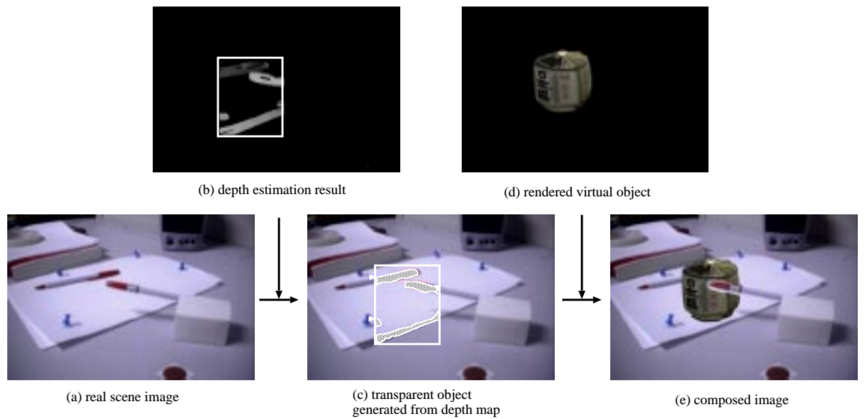
\includegraphics[width=1.0\textwidth]{content/images/methods/stereo-depth-map.png} 
  \caption{Visualisierung des Methode zur Vedeckung durch Depth Maps. Übernommen von \citet{kanbara2000stereoscopic}}
  \label{fig:stereo-depth-map}
\end{figure}

Als Erstes werden in diesem Verfahren 2D Bounding Boxen der zu rendernden virtuellen Objekte auf dem Viewport aus beiden Sichtfeldern der Stereokamera bestimmt. Die 2D Bounding Box wird durch eine Viewport Projektion der 3D Bounding Box eines virtuellen Objektes erzeugt. Diese Bounding Box Regionen wurden zunächst ermittelt, um die Bestimmung von Tiefeninformationen aus Performancegründen auf diese Bereiche zu beschränken. Als nächstes wird in den ermittelten Regionen ein Stereomatching mit Ecken aus der Anwendung des Sobel Filter durchgeführt. Hieraus können darauf folgend Tiefeninformationen der reellen Umgebung gewonnen werden. \citep{kanbara2000stereoscopic} \\

Da die Projekt Tango Hardware direkt Tiefeninformationen durch den Infrarot Laser liefert, wird das Stereomatching hier nicht weiter erläutert. Die Bestimmung von Bounding Boxen, wie von \citet{kanbara2000stereoscopic} beschrieben, ist somit auch nicht für die weitere Anwendung mit Project Tango relevant.\\


Um den Ausschluss der Pixel eines virtuellen Objektes, welches sich hinter einem reellen Objekt befinden, zu verhindern, wird der Z-Buffer Algorithmus nach \citet{greene1993hierarchical} angewendet. Dabei werden zunächst die ermittelten realen Tiefeninformationen in den Z-Buffer gefüllt. Das führt dazu, dass ein virtueller Bildpunkt des zu rendernden Objektes, welcher einen höheren Z-Wert als der bereits vorhandene Wert im Z-Buffer hat, also weiter vom Betrachter entfernt ist, nicht in den Framebuffer gelangt. In Abbildung \ref{fig:stereo-depth-map} ist das Vorgehen dieses Verfahrens noch einmal dargestellt, wobei im Fall von Project Tango Schritt \(b ) \) nicht angewendet wird. \\




\section{Echtzeit Polygon Rekonstruktion} \label{sec:polygon_reconstruction}

Die Idee der Verdeckung mit Hilfe des Z-Buffers lässt sich nicht nur direkten mit Depth Maps aus den Tiefenpunkten realisieren. Auch Primitiven oder allgemein Polygone könnten mit Hilfe eines entsprechenden Fragment Shaders, als Repräsentation der Umgebung, andere virtuelle Objekte Transparent überlagern, um die Illusion der Überdeckung von realen Objekten zu ermöglichen. Somit ließe sich das Problem der Optimierung von Augmented Reality mit Hilfe von Tiefeninformationen auf das Problem der Echtzeit Rekonstruktions zurückführen. \\

Die 3D Rekonstruktion ist bereits ein etabliert Forschungsgebiet in der Computer Grafik und gewinnt, auf Grund von kostengünstigen Consumer Tiefensensoren, wie die Microsoft Kinect, Asus Xtion oder Structure \citep{Struc48:online}, zunehmend an Bedeutung. Dabei wird sich immer mehr auf die Echtzeit Rekonstruktion konzentriert, da diese Geräte in der Lage sind, Tiefeninformationen, zwar mit leichten Messfehlern aber in Echtzeit, zu liefern. \citet{niessner2013real} erwähnen an dieser Stelle zudem den möglichen Einsatz für Augmented Reality:

\begin{quote}
\enquote{The ability to obtain reconstructions
in real-time opens up various interactive applications including:
augmented reality (AR) where real-world geometry can be fused
with 3D graphics and rendered live to the user; ...} \citep{niessner2013real}
\end{quote}

Die Herausforderung in der Echtzeit Rekonstruktion liegt dabei in der möglichst performanten Fusion von mehreren überlagernden Depth Maps. Hieraus soll eine möglichst detailierte Repräsentation der echten Umgebung generiert werden, welche sich im Idealfall stetig verbessert. Diese Problemstellung unterscheidet sich von herkömmlichen Rekonstruktionsverfahren wie die von \citet{hoppe1992surface} und der Poission Rekonstruktion von \citet{kazhdan2006poisson}. Aktuelle Verfahren nutzen dafür verschiedenste optimierte Datenstrukturen, welche zudem durch den Einsatz von entsprechenden GPU Implementierungen beschleunigt werden können. Dennoch spielt die Gegenüberstellung von Detailgrad, der Skalierung und Geschwindigkeit stets eine große Rolle. \citet{niessner2013real} \\

Bekannte Verfahren wie KinectFusion \citep{newcombe2011kinectfusion}, ein SLAM Verfahren von \citet{bylow2013real} oder DynamicFusion \citep{newcombe2015dynamicfusion} nutzen die \enquote{Truncated Signed Distance Function}, kurz TSDF, zur Speicherung und Migration der Oberflächeninformation mehrerer Depth Maps. Das Verfahren von \citet{niessner2013real} erweitert diesen Ansatz mit einem effizienten Spatial Hashing Verfahren, um die Zugriffszeiten und Speicherverbrauch zu minimieren. Darüber hinaus nimmt das Verfahren Chisel von \citep{Klingensmith_2015_7924} diese Vorzüge auf und kombiniert TSDF mit  \enquote{visual-inertial odometry}, der Trackingtechnologie von Project Tango. In den folgenden Absätzen werden die Mechanismen hinter TSDF, dem räumlichen Hashing und den Vorzügen von Chisel näher erläutert. Außerdem soll auch noch auf das Rendering der TSDF Oberfläche durch Marching Cubes eingegangen werden, welches in Chisel verwendet wird. \\


\subsection{Truncated Signed Distance Function}

Bei der von \citet{curless1996volumetric} vorgestellten räumlichen Repräsentation von Oberflächen, Truncated Signed Distance Function (TSDF), wird der Raum in Voxel einer gewünschten Auflösung unterteilt. Anders als Occupancy Maps, in denen die Voxel als sichtbar oder unsichtbar markiert werden, werden bei TSDF in den Voxeln die jeweiligen Entfernungen zur nächsten Oberfläche angegeben. Wichtig dabei ist das Vorzeichen, welches angibt, ob sich ein Voxel innerhalb oder außerhalb eines Objektes befindet. Abbildung \ref{fig:tsdf} zeigt unter a) die Ergebnisse mit Occupancy Maps und in b) die Voxel von TSDF. \citep{curless1996volumetric} \\

Gefüllt wird die Repräsentation durch die Depth Maps und der entsprechenden Kameraposition, die im Fall von Project Tango bereits gegeben ist. So wird für jede Tiefeninformation ein Strahl ausgehend von der Kameraposition generiert, der die durchgeschnittenen Voxel aktualisiert. Der Stahl ist dabei von der Länge begrenzt, um die zu aktualisierenden Voxel zu minimieren und zudem keine Oberflächen zu aktualisieren, die sich weiter hinter der gefundenen Oberfläche befindet. Dieses Vorgehen ist in Abbildung \ref{fig:tsdf} c) zu erkennen. \citep{Compu66:online} \\

\begin{figure}
  \centering
	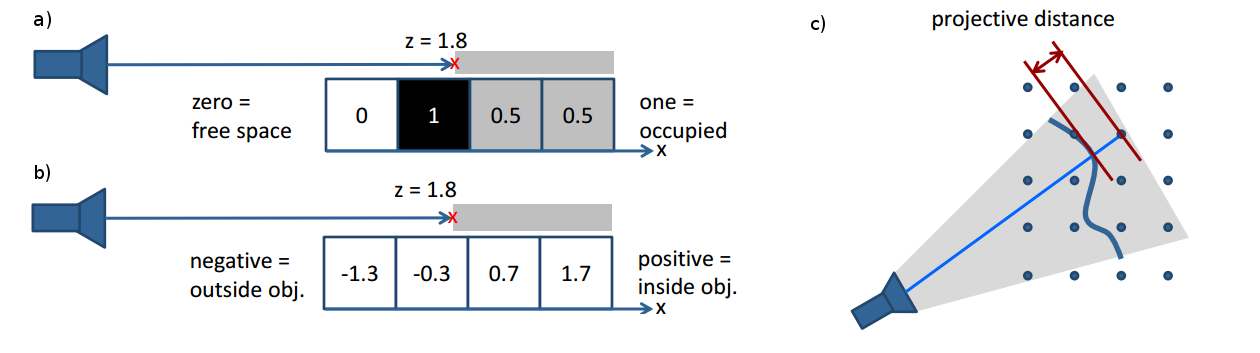
\includegraphics[width=1.0\textwidth]{content/images/methods/tsdf.png} 
  \caption{a) Beispielhafte Voxel Füllung von Occupancy Maps; b) Beispielhafte Voxel Füllung durch TSDF; c) Exemplarische 2D Darstellung der Oberfläche mit entsprechenden Strahlensatz für die TSDF. Übernommen von \citet{Compu66:online}}
  \label{fig:tsdf}
\end{figure}

Der Vorteil dieser Repräsentation liegt darin, dass die konkreten Oberflächeninformationen, anders als bei der Diskretisierung von Occupancy Maps, nicht verloren gehen. Das heißt, dass trotz einer gröberen Voxel Struktur stets der Nulldurchgang rekonstruiert werden kann. Neben der Entfernung zur nächsten Oberfläche wird zusätzlich noch ein Gewichtungswert in jedem Voxel gespeichert. Das ermöglicht es leichtes Rauschen durch einfache Mittelung zu unterdrücken und die Oberfläche optimiert sich somit bei jeder Aktualisierung der Voxel. \citep{Compu66:online}\\

\citet{hoppe1992surface} nutzen in Ihrem Rekonstruktionsverfahren auch die hier beschriebene TSDF. Jedoch bestimmen sie für jeden festgehaltenen Punkt der Pointcloud die umliegenden Nachbarn, um eine Tangentialebene zu ermitteln, von der aus die auf der Normalen liegenden Voxel mit der entsprechenden Distanz aktualisiert werden. Für die Echtzeitrekonstruktion ist dieses Vorgehen jedoch zu komplex. Hier werden die Voxel nicht anhand der exakten euklidischen Distanz aktualisiert, sondern es wird mit Hilfe des Raycastings, ausgehend von der Tiefenkamera, eine projizierte Distanz als Approximation verwendet. \citep{Compu66:online}

\subsection{Spatial Hashing}

Das Problem der Echtzeit Rekonstruktion ist wie bereits angesprochen der Kompromiss zwischen dem Detailgrad, der Skalierung der zu rekonstruierenden Szene und der Performance der Rekonstruktion. Auch die TSDF Repräsentation ist sehr speicherintensiv und benötigt für die zu scannende Szene reservierten Speicher, der auf mobilen Endgeräten nur begrenzt verfügbar ist. Daher muss auch für größere Rekonstruktionen oder Rekonstruktionen unbekannter Größe ein dynamischer Ansatz gefunden werden. \citet{Klingensmith_2015_7924} erwähnt dazu, dass einige Verfahren Octrees einsetzen, die zwar äußerst dynamisch sind, jedoch einen deutlichen Nachteil hinsichtlich der Zugriffszeiten auf die Voxel bergen. \\

\begin{figure}[h]
  \centering
	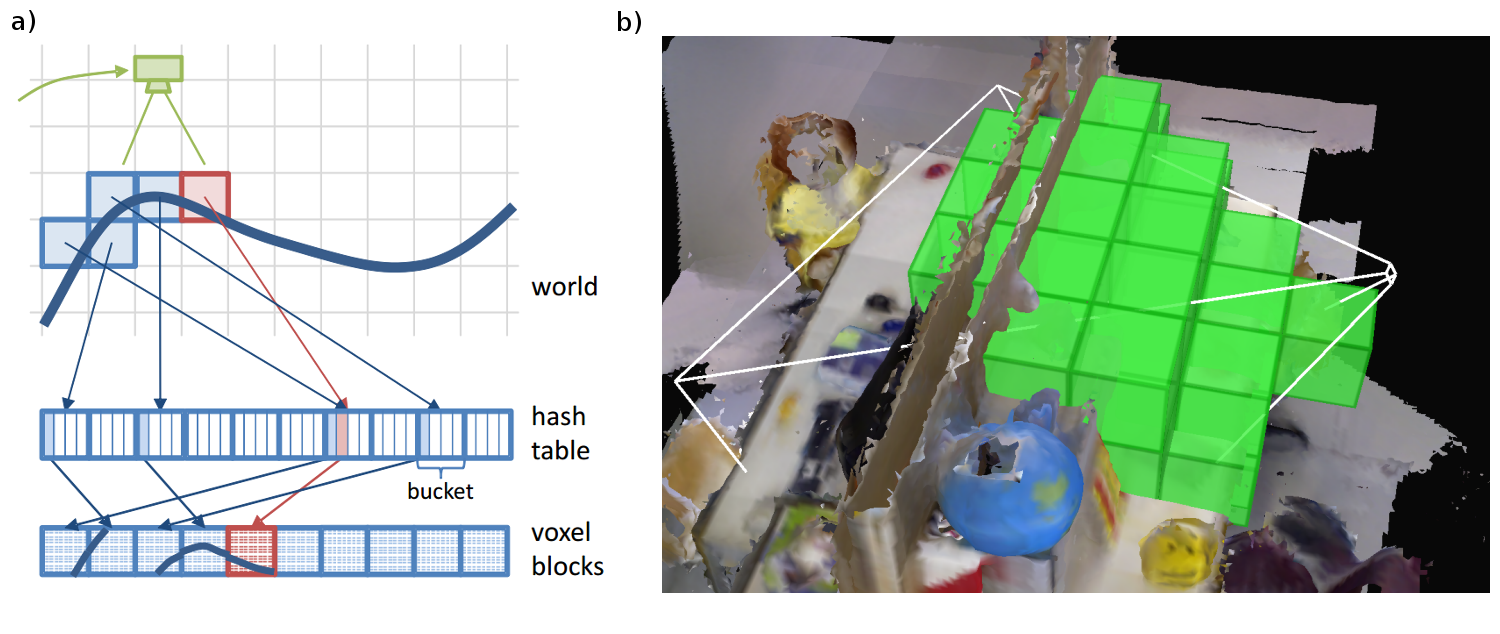
\includegraphics[width=1.0\textwidth]{content/images/methods/hashing.png} 
  \caption{a) Voxel Hashing Datenstruktur. Übernommen von \citet{niessner2013real} b) Darstellung der relevanten Voxel Chunks für die Aktualisierung. Übernommen von \citet{Klingensmith_2015_7924}}
  \label{fig:hashing}
\end{figure}

\citet{niessner2013real} führen daher eine zwei-Ebenen Struktur ein, die auf der zweiten Ebene eine Menge von Voxel räumlich zusammenfassen. Diese werden hier Chunks genannt. Auf der ersten Ebene können diese Chunks in einer Hash Tabelle räumlich mit einer Hashfunktion identifiziert werden. Das ermöglicht somit einen nahezu direkten Zugriff auf räumliche Voxel und ermöglicht es zudem Chunks dynamisch zu allokieren. Als Hash der Chunkposition \(x\), \(y\) und \(z\) wird die folgende Hashfunktion aus Gleichung \ref{eq:spatial_hash} verwendet. Bei den Variablen \(p_1\), \(p_2\) und \(p_3\) handelt es sich um willkürlich hohe Primzahlen und \(n\) entspricht der Größe der Hash Tabelle. 

\begin{equation}\label{eq:spatial_hash}
H(x,y,z) = (x * p_1 \oplus y * p_2 \oplus z * p_3) \mod n
\end{equation}

\subsection{Marching Cubes}

Die meisten Echtzeit Rekonstruktionen durch TSDF wie KinectFusion sind GPU Umsetzungen, die daher die Möglichkeit besitzen ein hardwarebeschleunigtes Rendering durch Raycasting durchzuführen. Das Verfahren Chisel von \citet{Klingensmith_2015_7924}, welches eine reine CPU Umsetzung ist, nutzt hingegen einen indirekten Weg zum Rendering durch die Marching Cubes Triangulation. \\

\begin{figure}[h]
  \centering
	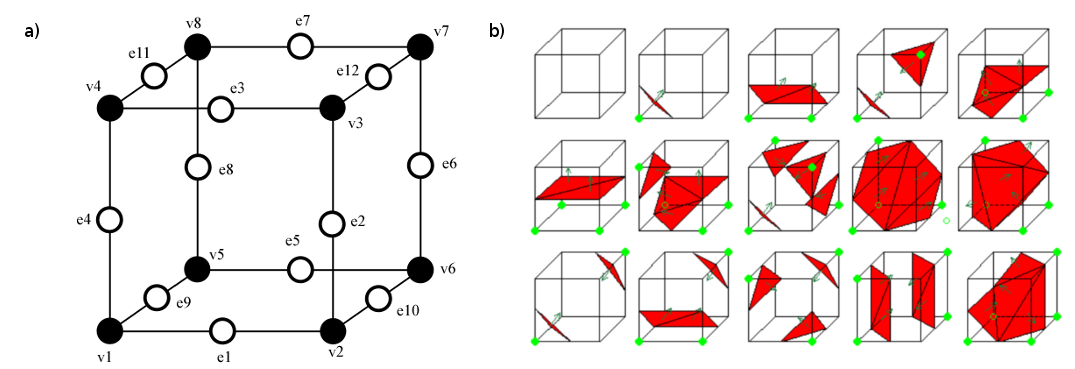
\includegraphics[width=1.0\textwidth]{content/images/methods/marchingcubes.png} 
  \caption{a) Marching Cubes Voxel Repräsentation mit den Ecken und den Kantenschnittpunkten b) Die 15 möglichen 3D Polygon Varianten. Übernommen von \citet{MarchingCubes:online}}
  \label{fig:marchingcubes}
\end{figure}

Marching Cubes nach \citet{lorensen1987marching} ist ein Algorithmus um aus einer, als Voxel repräsentierten, Isofläche Polygone zu bestimmen, die dieser Fläche möglichst nah kommt. Hierzu werden zu jedem Voxel die Ecken \(v1\) bis \(v8\) anhand der Nachbarvoxel und des Distanzwertes untersucht, ob sie innerhalb oder außerhalb eines Objektes liegen. Zusätzlich werden zu jeder Kante auf dem Voxel, wenn ein Schnitt der Isofläche existiert, die Schnittpunkte auf den Kanten \(e1\) bis \(e12\) bestimmt. Abbildung \ref{fig:marchingcubes} a) zeigt die Ecken und Kantenschnittpunkte eines Voxels. \\

Je nach binärer Gewichtung der Ecken können hiernach aus einem Katalog von 256 Varianten die Polygone nachgeschlagen werden. Inhalt des Katalogs sind die Indizes der Kantenschnittpunkte, aus denen Polygone generiert werden können. Alle diese 256 Varianten können auf 15 verschiedene Fälle zurückgeführt werden, die sich nur in Rotation oder Symmetrie unterscheiden. Die 15 Varianten sind in Abbildung \ref{fig:marchingcubes} b) zu finden. \citep{MarchingCubes:online} \\

\subsection{Chisel mit Space Carving}

Das Bereits erwähnte Verfahren Chisel von \citet{Klingensmith_2015_7924} verwendet alle zuvor erwähnten Techniken der TSDF, spatial Hashing und der Marching Cubes Überführung. Sie sprechen dabei von einem \enquote{dynamic spatial-hashed truncated distance field}. Das für den mobilen Einsatz optimierte Verfahren ist in der Lage eine Echtzeitrekonstruktion von Räumen von bis zu \(300 m^2\) mit einem Detailgrad von zwei bis drei Zentimetern zu erstellen. Zudem können neben Tiefeninformationen auch gefärbte Pointclouds verarbeitet werden, wodurch ein gefärbtes Mesh generiert werden kann. \citep{Klingensmith_2015_7924}\\

Zusätzlich erweitern sie den TSDF Algorithmus um die \enquote{space carving} Funktionalität. Sie betrachten dabei den Strahl von der Kamera zur Oberfläche als eine Art Constraint, in dem alle durchstoßenden Voxel bis zur Oberfläche eine negativen Wert beinhalten müssen. Ist das nicht der Fall, so wird ein Voxel außerhalb der inneren Begrenzung auf den leeren Ursprungswert gesetzt. Im Pseudocode aus Listing \ref{lst:chisel} wird das Verhalten näher erläutert. Diese Verbesserung führt dazu, dass die Rekonstruktion bei stark rauschenden Tiefeninformationen, besonders an Objektkanten, deutlich verbessert wird. Außerdem ist das Verfahren hiermit in der Lage dynamische Änderungen in der Umgebung zu detektieren und neue Oberflächen entsprechend zu aktualisieren. So beeinflussen zum Beispiel sich im Bild bewegen Personen nur kurz die Voxel der TSDF. \citep{Klingensmith_2015_7924}\\

\begin{lstlisting}[mathescape,caption=Chisel TSDF Algorithmus, label=lst:chisel]
Eingabe: Pointcloud $C$, Kameratransformation $P_{cam}$, 
         Strahlenbegrenzung $t$

für jeden Tiefenwert $\vec{p}$ aus $C$
    bestimme die Oberflächenposition $\vec{z}$ aus $\vec{p}$ und $P_{cam}$
    bestimme einen Strahl $\vec{r}$ aus $\vec{z}$ und $P_{cam}$
    bestimme den Begrenzungsbereich $t_{vor}$, $t_{nach}$ mit $t$ um $\vec{z}$ auf $\vec{r}$
    # space carving
    für jeden Voxel $v$ zwischen Kamera und $t_{vor}$
        wenn die Distanz im Voxel negativ ist
            setze Voxel zurück
    # normale TSDF Bestimmung
    für jeden Voxel $v$ zwischen $t_{vor}$ und $t_{nach}$
        bestimme die Voxeldistanz zu $z$
        setze das Gewicht w des Voxels $v$
\end{lstlisting}

Neben space carving wurden zudem eine variable Strahlenbegrenzungen und Gewichtungen der Voxel abhänig von der jeweils aufgenommenen Tiefe implementiert. Diese Funktion berücksichtigt die Varianzen von Messungenauigkeiten des Sensors, die bei größerer Entfernung der Oberfläche zum Tiefensonsor zunehmen können. \citep{Klingensmith_2015_7924}

\textbf{TODO:} DARSTELLUNG DES STRAHLS, DER KAMERA UND DER OBERFLÄCHE ZUR VERSTÄNDNIS DES ALGORITHMUS

\section{Planare Rekonstruktion} \label{sec:plane-reconstruction}

Dieses Kapitel widmet sich der Idee, eine Rekonstruktion für ein Rekonstruktions basiertes Überlagerungsverfahren durch eine Ebenendetektion zu realisieren. \citet{yang2010plane} erwähnt hierzu, dass Ebenen in fast allen künstlichen Umgebungen zu finden sind und auf Grund ihrer vorteilhaften geometrischen Eingenschaften in verschiedensten Computer Vision Verfahren verwendet werden. Daher gibt es viele Forschungsarbeiten, Methoden und Algorithmen, um aus verschiedensten Informationsquellen ein Ebenenmodell zu extrahieren.\\

Das \enquote{Simultaneous Localization and Mapping} (SLAM) Verfahren von \citet{trevor2012planar} detektiert Ebenen mit dem RANSAC Algorithmus. RANSAC bietet gegenüber anderen Algorithmen zur Ebenen Detektion den Vorteil, ein Modell auch bei vielen Ausreißern performant zu ermitteln. Agglomeratives Clustering und Region Growing wie von \citet{feng2014fast} beschreiben, eignet sich auf Grund des Ausgabeformats von Project Tango nicht direkt, da es keine organisierte Point Cloud ausgibt und die Daten durch Reflektionen und Löchern mit Fehlern behaftet sind. \\

Das selbst zusammengestellte Verfahren zur Ebenendetektion besteht daher aus folgenden Komponenten. Wie in dem Ansatz von \citet{yang2010plane} wird der RANSAC Algorithmus auf Würfeln ausgeführt, die eine Menge gesammelter Punkte aus der Pointcloud beinhaltet. Dabei entsprechen die Würfel den untersten Knoten eines Octrees, welcher hier zur Speicherung und Aufnahme aller Punkte verwendet wird. Eine gefundene Ebene in einem Würfel wird wie im SLAM Verfahren von \citet{trevor2012planar} persistiert. Die Repräsentation der Ebene \(P\) wird dort wie in Gleichung \ref{eq:plane} festgehalten. Dabei handelt es sich um den Normalenvektor \(\vec{n}\) und der Distanz zum Ursprung \(d\) der Hesse Normalform einer Ebene, sowie der Punkte der konvexen Hülle \(H\). \citet{trevor2012planar} erläutern, dass die konvexe Hülle in der Repräsentation festgehalten wird, um eine sukzessive Verbesserung einer Ebene nach mehreren Messdurchläufen zu ermöglichen. So werden die Punkte der konvexen Hülle pro Messvorgang kombiniert, damit die Ebenenausbreitung auch außerhalb des Sichtfeldes beibehalten werden kann. \\

\begin{equation} \label{eq:plane}
P=\left[\vec{n}, d, H\right] \qquad H=\vec{h_1}, \vec{h_2}, \ldots  \vec{h_n}
\end{equation}

Die einzelnen Schritte des Vorgehens werden in den folgenden Absätzen näher erläutert. Ein grober Ablauf des Vorgehens wird aber bereits in Listing \ref{lst:planeReconstruction} zusammengefasst und in Pseudocode beschreiben. Als Cluster sind im Listing sind die untersten Nodes eines Octrees gemeint.

\begin{lstlisting}[mathescape,caption=Planare Echtzeit Rekonstruktion, label=lst:planeReconstruction, float=htbp]

Eingabe: Octree $O$, Anzahl der zu suchenden Ebene in Clustern $N$
Ausgabe: Polygonpunkte $T_{Gesamt}$

für jedes Cluster $C$=[$C_{Punkte}$, $C_{Ebenen}$] aus $O$
    führe $N$ mal aus
        bestimme Ebene [$\vec{n}$, $d$, $P$] mit RANSAC aus $C_{Punkte}$
        wenn keine Ebene mit genügend $P$ gefunden wurde
            nächstes Cluster (continue)
        wenn Ebene mit [$\vec{n}$, $d$, $H_{alt}$] in $C_{Ebenen}$ existiert	
            füge die konvexe Hülle $H_{alt}$ zu $P$ hinzu	
        bestimme die konvexe Hülle $H_{neu}$
        trianguliere $H_{neu}$ zu $T_{Ebene}$
        $T_{Gesamt}$ += $T_{Ebene}$
        $C_{Ebenen}$ += [$\vec{n}$, $d$, $H_{neu}$]
        $C_{Punkte}$ - $P$
\end{lstlisting}


\subsection{RANSAC zur Ebenendetektion} \label{sec:ransac}

Um mit dem RANSAC Algorithmus, beschrieben in Kapitel \ref{sec:ransac-theory}, Ebenen in einer Punktewolke bestimmen zu können, werden pro Iteration drei Stichproben \(\vec{A}\), \(\vec{B}\) und \(\vec{C}\) gewählt, die zur Bestimmung einer Ebene ausreichen. Das Ebenenmodell, hier in der Hesse Normalform mit dem Normalenvektor \(\vec{n}\) und dem Abstand zum Koordinatenursprung \(d\), lässt sich dabei durch die Gleichung \ref{eq:normalform} bestimmen.

\begin{equation}\label{eq:normalform}
\vec{n} =\left|\left| \vec{AB} \times \vec{AC}\right|\right|
\qquad
d = \vec{A} \cdot \vec{n}
\end{equation}

Um zu ermitteln ob ein Punkt \(\vec{P}\) aus einer Messreihe die gefundene Ebene \(\left[\vec{n}, d\right]\) unterstützt, wird die kürzeste Distanz \(d_P\) zwischen Punkt und Ebene wie in Gleichung \ref{eq:plane-distance} ermittelt.  Ein entsprechender Toleranzwert für die Distanz \(d_{min}\), im gezeigten RANSAC Algorithmus \(e\) genannt, wird später bei der Umsetzung abhängig von der Ungenauigkeit des Tiefensensors gewählt. 

\begin{equation} \label{eq:plane-distance}
d_P = \vec{n} \cdot \vec{P} - d \qquad support_{d_P} = d_P < d_{min}
\end{equation}

Um das finale Modell der Ebene zu ermitteln, wie im Ursprünglichen RANSAC Algorithmus in Punkt 7. beschrieben, und somit die Varianz des Abstands der Punkte zur Ebene zu minimieren, wird mit Hilfe der unterstützenden Punkte \(P_{s}=\left[x,y,z\right]\) eine lineare Regression durchgeführt. Diese Mittelt ein Ebenenmodell \(E=\left[\vec{n}, d\right]\) aus den zuvor ermittelten Punkten mit Hilfe der Methode der kleinsten Quadrate. \citet{hoppe1992surface} nutzen hierfür für eine ähnliche Problemstellung die Eigenwert Dekomposition der Kovarianzmatrix der Punkte \(P_{s}\) zum Zentrum \(\vec{p_{c}}\). In Gleichung \ref{eq:centroid} wird das Zentrum aus den unterstützenden Punkten \(P_{s}\) bestimmt. Gleichung \ref{eq:covarianz} zeigt die Bestimmung der Kovarianzmatrix \(CV\) im Bezug zum Zentroid, in der \(\otimes\) für das dyadische Produkt\footnote{Wenn \(\vec{a}\) und \(\vec{b}\) die Komponenten \(a_i\) und \(b_j\) beinhalten, resultiert aus \(\vec{a} \otimes \vec{b}\) eine Matrix mit den Komponenten \(a_ib_j\) an der \(ij\) Position. \citep{hoppe1992surface}} steht.

\begin{equation} \label{eq:centroid}
\vec{p_{c}} = \frac{\sum_{n=0}^{|P|} P_{n}}{|P|}
\end{equation}

\begin{equation} \label{eq:covarianz}
CV = \sum_{n=0}^{|P|} ( \vec{p_{n}}- \vec{p_{c}}) \otimes ( \vec{p_{n}}- \vec{p_{c}})
\end{equation}

Wendet man nun auf der Kovarianzmatrix \(CV\) die Eigenwert Dekomposition an, erhält man die Normale \(\vec{n}\) aus dem Eigenvektor \(||\vec{v_i}||\) mit dem kleinsten Eigenwert \(\lambda_i\). Somit würde bei \(\lambda_1 \geqq \lambda_2 \geqq \lambda_3\) die Zuweisung \(\vec{n} = ||\vec{v_3}||\) folgen. Die Distanz zum Ursprung \(d\) entspricht dem Kreuzprodukt aus dem Zentroiden \(\vec{p_c}\) und der neu gewonnen Normalen \(\vec{n}\). \citep{hoppe1992surface} \\

\subsection{Bestimmung der Ebenenausbreitung}

Nachdem die Ebene und die korrespondierenden Punkte zur Ebene gefunden wurden, muss noch die Ausbreitung der Fläche bestimmt werden, da die Ebene in Hesse Normalform lediglich die Position \(\vec{n} * d\) und Ausrichtung \(\vec{n}\) festhält. \citet{PlanarSurfaceMapping} nutzt hierfür die konvexe Hülle der korrespondierenden Punkte und trianguliert diese. Wie diese dort genau bestimmt wurde ist nicht beschrieben. \\

Um diese Bestimmung performant umsetzen zu können, kann man sich hier die Eigenschaft der Ebene zu Nutzen machen und die dreidimensionalen Punkte durch Parallelprojektion als zweidimensionale Punkte auf die Ebene projizieren. Denn die Triangulation ist nach dem Erhalten der zweidimensionalen konvexen Hülle, wie im Listing \ref{lst:triangulation} beschrieben, direkt bestimmbar. Nach der Triangulation können die Ecken der gefundenen Polygone jeweils zurück projiziert werden. Die Gleichungen \ref{eq:projection2d} und \ref{eq:projection3d} bilden die Projektion der Punkte wobei \(R_{\vec{n} \rightarrow \vec{z}}\) der Rotationsmatrix zwischen dem Normalenvektor \(\vec{n}\) und der Z-Achse \(\vec{z}\) entspricht.\\

\begin{equation} \label{eq:projection2d}
p_{2d} = (p_{3d} - (\vec{n}*d)) * R_{\vec{n} \rightarrow \vec{z}}
\end{equation}
\begin{equation} \label{eq:projection3d}
p_{3d} = (p_{2d} * R_{\vec{n} \rightarrow \vec{z}}^{-1}) + (\vec{n}*d)
\end{equation}

\begin{lstlisting}[mathescape,caption=Bestimmung der Ebenenausbreitung und Triangulation, label=lst:triangulation, float=htbp]

Eingabe: Unterstützende Ebenenpunkte aus RANSAC $P$
         Transformation $R_{\vec{n} \rightarrow \vec{z}}$
Ausgabe: Polygone $T_{Ebene}$

    Projiziere alle Punkte aus $P_s$ mit $R_{\vec{n} \rightarrow \vec{z}}$ zu $P_{2d}$
    Bestimme die konvexe Hülle $H$ aus $P_{2d}$ mit Graham Scan
    starte mit leerer Menge $P_{2dmesh}$
    für $i$ von $0$ bis $|H| - 2$
        füge $H_i$ zu $P_{2dmesh}$ hinzu
        füge $H_{i+1}$ zu $P_{2dmesh}$ hinzu
        füge $H_{i+2}$ zu $P_{2dmesh}$ hinzu
    Projiziere alle Punkte aus $P_{2dmesh}$ mit $R_{\vec{n} \rightarrow \vec{z}}^{-1}$ zu $P_{3dmesh}$
   
\end{lstlisting}


\subsection{Clustering der aufgenommenen Punkte} \label{sec:cluster}

Wie im Listing \ref{lst:planeReconstruction} zu erkennen wird das zuvor beschriebene Vorgehen für die planare Rekonstruktion immer pro Cluster eines Cluster-Pools durchgeführt. Dadurch werden pro Durchgang des Algorithmus nur ein Bruchteil der gesammelten Punkte rekonstruiert, was wiederum eine Rekonstruktion in Echtzeit möglich macht. Außerdem verhindert das Clustering das Bilden von konvexen Hüllen über Ebenen, die in Zwischenbereichen nicht mit genügend Punkten unterstützt werden. Dieses Problem ist in Abbildung \ref{fig:clustering} links zu sehen, in welcher eine blaue Ebene Rekonstruiert wird, die sich über einen Durchgang ohne vorhandene Punkte streckt.\\

\begin{figure}[h]
  \centering
	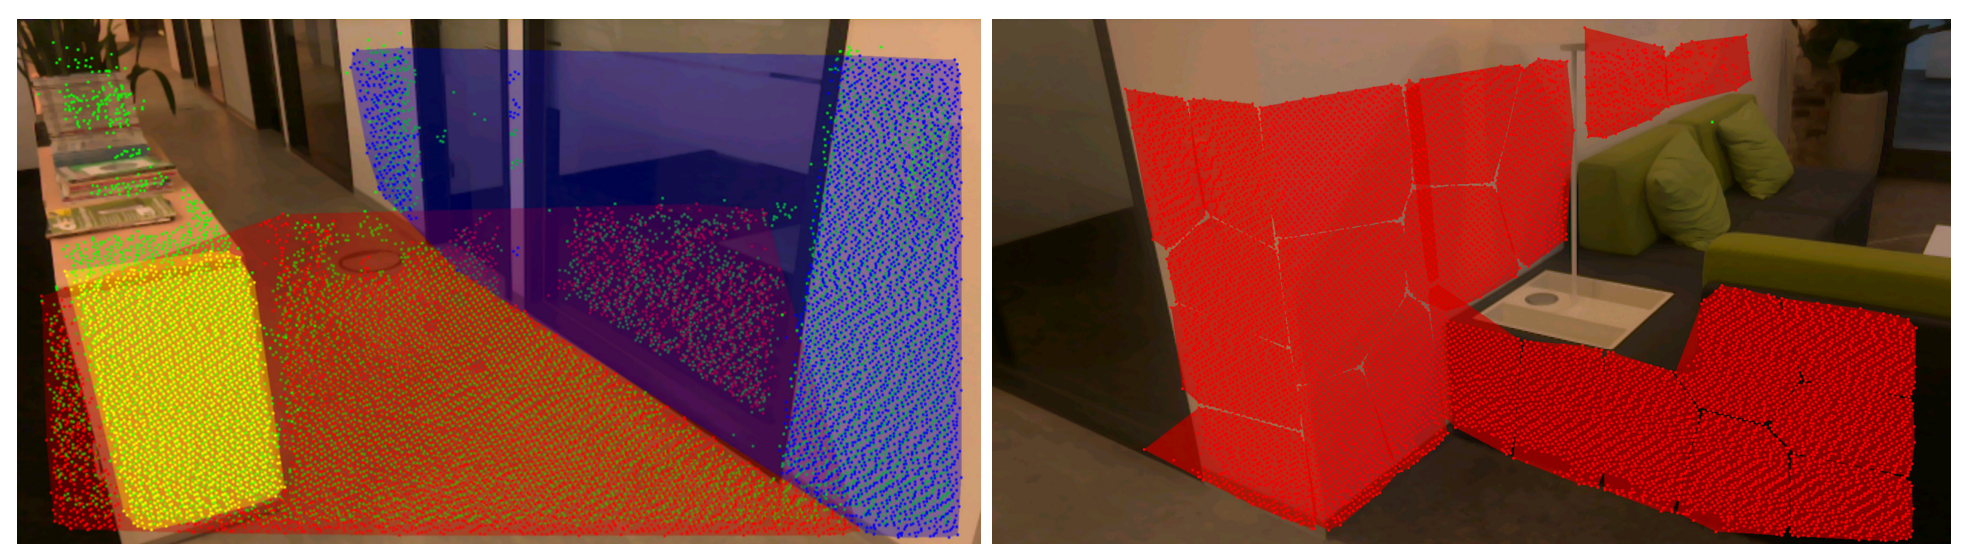
\includegraphics[width=1.0\textwidth]{content/images/methods/clustering.png} 
  \caption{Links: Ebenenrekonstruktion ohne Clustering. Rechts: Rekonstruktion mit K-Mean Clustering.}
  \label{fig:clustering}
\end{figure}

Getestet wurden hier das K-Mean Clustering, Agglomeratives Clustering und einfaches räumliches Clustern mit Hilfe eines Octrees. Das K-Mean Clustering hat, wie in Abbildung \ref{fig:clustering} rechts zu erkennen, gute Ergebnisse für die Aufteilung einer Ebenen geliefert, benötigt aber zuvor eine feste Anzahl von Clustern. Agglomeratives Clustering, getestet mit dem euklidischen Distanzmaß, würde zwar die Anzahl der Cluster dynamisch bestimmen, ist jedoch zu aufwändig für eine Echtzeit Rekonstruktion. \\

Gute Ergebnisse liefert wiederum ein einfaches räumliches Clustern mit einem Octree, welcher die aufgenommenen Punkte direkt in Knoten des Baums zuweist. Das bietet zudem den Vorteil, dass diese Datenstruktur direkt als Speicherort der Aufgenommenen Punkte und Ebenen dienen kann. Außerdem entspricht dies dem Vorgehen für die Anwendung von RANSAC auf Würfeln, welches von \citet{yang2010plane} beschrieben wurde. \\


\section{Tiefenanpassungen durch Farbbilder}

Aus allen zuvor beschriebenen Verfahren werden letztendlich Tiefeninformationen, in Form von geometrischen Primitiven oder Punkten im Raum gewonnen. Diese werden passend zur aktuellen Kameraposition als Tiefenbild gerendert und füllen den Z-Buffer für eine entsprechende Aussparungen bei der Überdeckung virtueller Objekte. Auf Grund von Sensorungenauigkeiten und den daraus resultierenden größeren Auflösungen der Rekonstruktionsverfahren können dabei fehlerhafte Tiefeninformationen im Z-Buffer gelangen, die zu Fehlern bei der Bestimmung der Überdeckung führen können. Dieses Problem ist am Beispiel der Pointcloud Projektion aus Kapitel \ref{sec:pc-projection} in Abbildung \ref{fig:pc-noise} zu erkennen. \\

\begin{figure}[h]
  \centering
	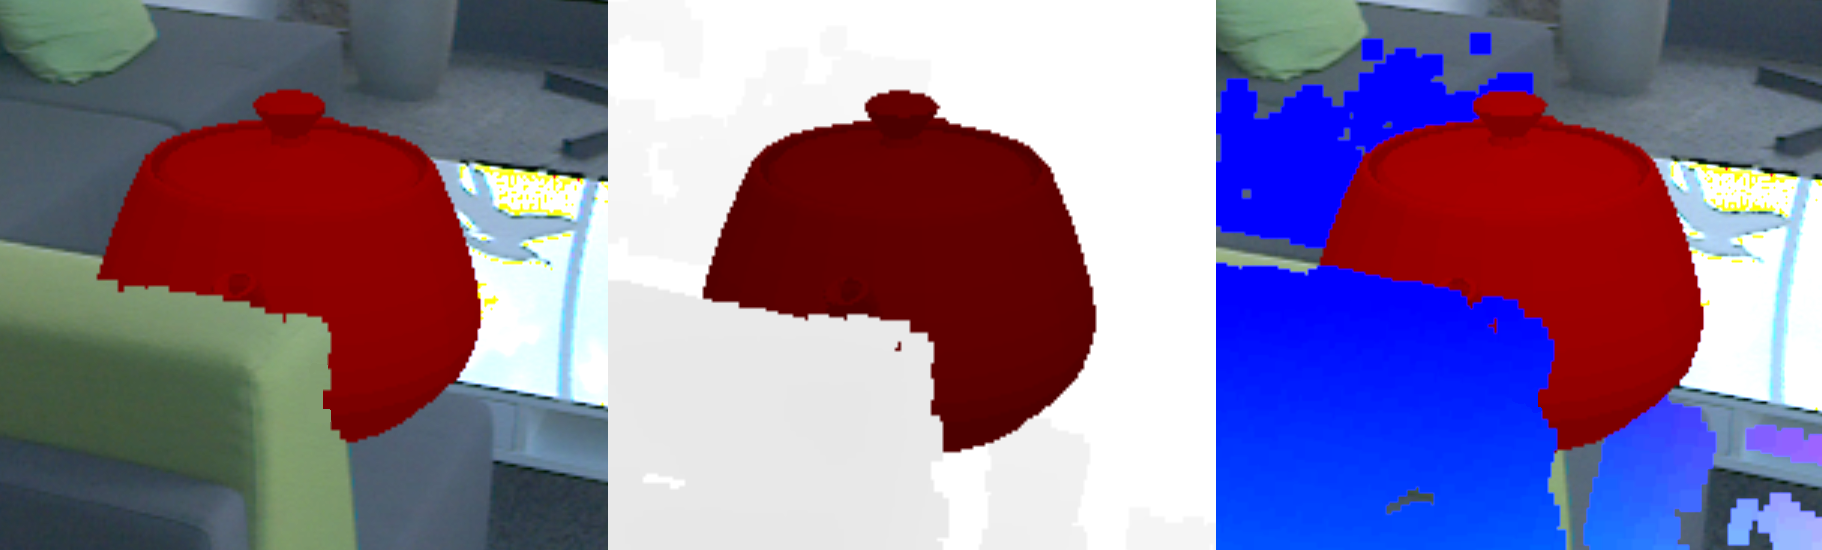
\includegraphics[width=1.0\textwidth]{content/images/methods/pc-noise.png} 
  \caption{Überdeckung mit einfacher Pointcloud Projektion. Links: Resultat der Überdeckung. Mitte: Darstellung des Tiefepuffers. Rechts: Darstellung der Pointcloud.}
  \label{fig:pc-noise}
\end{figure}

Die Reduktion von Ungenauigkeiten im Tiefenbild könnte durch einen Gaußschen Weichzeichner erreicht werden. Dieser würde jedoch die Kanten im Farbbild nicht berücksichtigen und somit fehlerhafte Tiefen Gradienten an den Kanten erzeugen. \citet{newcombe2011kinectfusion} wenden einen sogenannten \enquote{Bilateralen Filter} in ihrem KinectFusion System an, bevor sie die Tiefeninformationen in die TSDF Repräsentation einfließen lassen. Dieser Filter von \citet{tomasi1998bilateral} ermöglicht das Weichzeichnen ohne dabei die Kanten im Bild zu übergehen, bezieht sich jedoch nur auf das selbe Bild, auf dem der Filter angewendet wird. \\

\citet{liu2012guided} hingegen wenden einen sogenannten \enquote{Guided Filter} in Ihrem Verfahren zur Optimierung der der Tiefeninformationen für Kinect ähnliche Sensoren auf das Tiefenbild an. Dieser Filter von \citet{he2010guided} ist in der Lage, auf Grundlage eines anderen Leitbildes ein Weichzeichnen durchzuführen, ohne dabei die Kanten des Leitbildes zu überschreiten. Auch wenn \citet{petschnigg2004digital} eine Erweiterung, den Joint Bilateral Filter, vorstellen, der auf Basis eines Leitbildes eine Weichzeichnung ohne Kantenüberschreitung ermöglicht, bietet der Guided Filter eine deutlich bessere Performance. Außerdem verhindert der Guided Filter Fehler Artefakte im Resultat, die bei dem Bilateralen Filter an den Kanten auftreten können. \citep{he2010guided}

\section{Interaktion mit Tiefeninformationen durch Raypicking} \label{sec:ar-depth-interaction}

Wie in Kapitel \ref{sec:ar-interaction} beschrieben, bedarf es bei der Umsetzung von Augmented Reality Systemen ein anderes Interaktionsparadigma. Auch wenn die Entwicklung der neuen Tablet und Smartphone Geräte durch Touchscreens eine neue Interaktionsform eingeführt haben, ist sie in den meisten Fällen auf einer zweidimensionalen Ebene beschränkt. In der Entwicklung von Virtual Reality oder voll virtuellen Anwendungen und Spielen wird oft für die Auswahlgeste der Raypicking Mechanismus verwendet, um eine zweidimensionale Interaktion im dreidimensionalen Raum zu ermöglichen. Darüber hinaus gibt es verbesserte semantische Interaktionsformen basierend auf einer zweidimensionalen Toucheingabe, wie von \citet{elmqvist2008semantic} beschrieben.\\

Hier soll aber zunächst eine Raycasting Variante für Augmented Reality Anwendungen umgesetzt werden, die nicht von einem kompletten Modell in Form von Polygonen oder anderen Primitiven der realen Umgebung ausgeht. Diese AR Interaktionsmöglichkeit ermöglicht, anhand der Tiefeninformationen, das passende Positionieren von virtuellen Objekten im realen Raum und lässt sich auf weitere Interaktionen erweitern. Voraussetzung für die folgende Umsetzung, ist die entsprechende Kalibrierung und Gleichstellung der extrinsischen und intrinsischen Kameraparametern der virtuellen sowie der realen Kamera. \\

\begin{figure}[h]
  \centering
	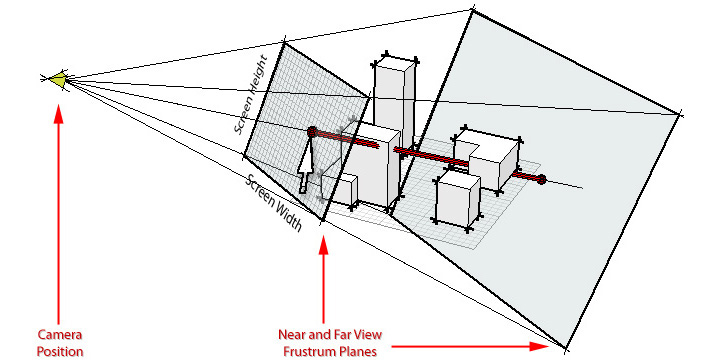
\includegraphics[width=1.0\textwidth]{content/images/methods/interaction.jpg} 
  \caption{Raypicking Visualisierung. Übernommen von \citet{gluUn11:online}}
  \label{fig:interaction}
\end{figure}

Als Erstes wird ein Strahl erzeugt, der durch die Position der virtuellen Kamera und durch den jeweils ausgewählten Punkt auf der Viewingplane läuft. Den Ursprung der virtuellen Kamera bestimmt dabei Google Tangos \enquote{Motion Tracking}. Der gewählte beziehungsweise berührte Punkt auf dem Touchscreen wird dabei zunächst von Pixeln in das Verhältnis \(\left[-1,1\right]\) des Punktes umgerechnet. Hiernach wird die Projektion auf die Viewingplane durch eine Multiplikation mit \(T\) aus Gleichung \ref{eq:unprojection} rückgängig gemacht. Der Gerade aus den beiden Punkten kann danach genutzt werden, um den Schnitt von Objekten vor der Kamera zu ermitteln. \citep{OpenG86:online} 

\begin{equation} \label{eq:unprojection}
T  = MV_{ModelView}^{-1} * P_{Projection}^{-1}
\end{equation}

Angewendet auf die Tiefeninformation aus Tangos \enquote{Depth Perception} wird die Punktewolke, wie in Abbildung \ref{fig:interaction}, vor die Kamera projiziert. In den projizierten Punkten wird danach der entsprechende Punkt gesucht, welcher sich am nächsten am zuvor bestimmten Strahl befindet. Durch diese beschriebenen Schritte kann der Nutzer mit einer zweidimensionalen Geste einen Punkt in der Tiefe bestimmen.



% Umsetzung
\chapter{Implementierung}

Dieses Kapitel widmet sich der Umsetzung der in Kapitel \ref{sec:optimization} beschriebenen Verfahren. Hierfür wurden im Laufe dieser Arbeit verschiedene Prototypen entwickelt, die jeweils als Proof of Concept für die einzelnen Verfahren galten. Ziel dieser Umsetzung ist es einen einzigen Prototypen in Form einer App auf dem Project Tango Gerät zu entwickeln, die den gesamten Funktionsumfang, welcher in Kapitel \ref{sec:final_prototype} zusammengefasst wird, beinhaltet. \\

Zudem muss ein Programmfluss geschaffen werden, der es ermöglicht, in die Daten des Tiefenbuffers mit eigenen Implementierungen eingreifen zu können, um ein Filtern zu ermöglichen. Wie das technisch ermöglicht wird, und auf welcher Basis die Anwendung implementiert wird, beschreibt das Kapitel \ref{eq:technic}. Hiernach werden die Umsetzung der die jeweiligen Verfahren näher erläutert.

\section{Finaler Prototyp} \label{sec:final_prototype}

Der finale Prototyp soll, wie bereits erwähnt, alle zuvor beschriebenen Verfahren zur Realisierung von Überlagerungen in einer Augmented Reality Szene beinhalten. Also muss zunächst eine einfache AR Szene geschaffen werden, in der eine virtuelle Kamera existiert, die die intrinsischen und extrinsischen Eigenschaften der Project Tango Kamera zu jeder Zeit entspricht. Außerdem muss das aktuelle Farbbild der RGB Kamera in der Szene im Hintergrund dargestellt werden. Für diese Aufgaben existieren, wie bereits in Kapitel \ref{sec:theory_project_tango} erwähnt, Schnittstellen, die diese Informationen liefern. \\

Um eine reale Überdeckung sinnvoll testen zu können, benötigen wir zudem ein virtuelles Objekt in der Szene. Dieses sollte im Idealfall nicht zu einfach gestaltet sein, damit die Verfahren anhand realistischen Gegebenheiten verglichen werden können. Zu diesem Zweck sollen Objekte in die App eingelesen werden können, die in in dem Forschungsbereich der Computergraphik typischerweise eingesetzt werden. Typische Modelle sind zum Beispiel der \enquote{Utah Teapot}, \enquote{Stanford Bunny} oder \enquote{Blenders Suzanne}\footnote{List of common 3D test models - https://goo.gl/MsOtSW}.  Eines dieser Modelle soll in die Szene geladen werden und es soll die Möglichkeit gegeben sein, dass das Objekt flexibel positioniert werden kann. Hierzu wird zudem der beschriebene Raypicking Mechanismus umgesetzt.\\

Um die Ergebnisse der  realen Überlagerung einfach gegenüberstellen zu können, sollen die beschriebenen Tiefenbild generierenden Verfahren flexibel im Betrieb ausgetauscht werden. Dazu gehört das Rendering der Pointcloud Projektion, die TSDF Rekonstruktion durch Chisel und die Ebenen Rekonstruktion. Außerdem soll das Filtern des Tiefenbildes mit Hilfe des Guided Filter optional zu jeder Zeit möglich sein. Hilfreich wäre es zudem, die Einstellungen des Guided Filters flexibel einstellen zu können. Wie diese Verfahren und ihre Flexibilität umgesetzt wird in den folgenden Kapiteln näher beschrieben.

\section{Technische Umsetzung und Struktur} \label{eq:technic}

Wie bereits erwähnt, basiert das Project Tango System auf Googles Android Betriebsystem. Dies ermöglicht es Anwendungen mit bestehenden und bewerten Technologien wie OpenGL, Rajawali\footnote{Android OpenGL ES 2.0/3.0 Java Engine - https://goo.gl/r9Ohdj (27.02.16)} oder der Unity Engine entwickeln zu können. Project Tango bietet hierfür drei verschiedene Schnittstellen, in C/C++, Java und Unity (Mono Framework in C\#), um auf die Sensordaten in verschiedenen Umgebungen zugreifen zu können. Im laufe dieser Arbeit wurden alle Schnittstellen mit verschiedensten prototypischen Entwicklungen getestet.\\

Der finale Prototyp wurde letztendlich in C/C++ entwickelt und basiert auf dem Android NDK\footnote{Android Native Development Kit - http://goo.gl/ananZT (27.02.16)}. Letztendlich greifen die anderen, höher angesiedelten Schnittstellen auf genau die selbe native Implementierung zurück, um sie in Java und Unity zu Verfügung zu stellen. Außerdem ermöglicht die native Entwicklung, neben Performancevorteilen, den vollen Zugriff auf OpenGL Mechanismen, die von Rajawali gegebenenfalls ausgeschlossen werden. \\

Das Projekt Tango Team stellt für die native Entwicklung die eigentliche Tango Schnittstellen Bibliothek\footnote{Project Tango C API - https://goo.gl/lbBfAp (27.02.16)}, eine Support-Bibliothek\footnote{Project Tango C Suppport API - https://goo.gl/VGyeKm (27.02.16)} und eine einfache Kapselung für OpenGL Anwendungen mit dem Namen TangoGL\footnote{TangoGL Repository - https://goo.gl/ymDCsJ (27.02.16)} an. Die Support-Bibliothek bietet verschiedene Hilfsfunktionen zur Datenverarbeitung und Allokation. TangoGL wiederum erleichtert den Einstieg in die OpenGL Entwicklung und übernimmt die Grundlegende Struktur und Interoperabilität zu Project Tango. Zum Beispiel gibt es Methoden, um Tango Positionsdaten in eine Translationsmatrix umrechnen zu können oder Klassen, die das Rendern der aktuellen RGB Kamera Textur übernehmen. \\

Abbildung \ref{fig:structure} zeigt grob den strukturellen Aufbau der Android Applikation. Der obere Teil der Grafik bezieht sich dabei auf den in Java implementierten Teil, der die Nutzeroberfläche, ihre Interaktion und den Renderingcanvas beinhaltet. Die Activity stellt jedoch nur einen kleinen Teil der Anwendung dar, denn alle Interaktionen und Ereignisse werden über ein Java Native Interface (JNI) zum nativen Teil der Anwendung geleitet, welcher die Ansprache der Schnittstellen, die Prozesslogik und das Rendering selbst beinhaltet. \\

\begin{figure}[h]
  \centering
	\includegraphics[width=1.0\textwidth]{content/images/implementation/uml.png} 
  \caption{Struktureller Aufbau des Prototypen}
  \label{fig:structure}
\end{figure}

Die Hauptklasse \enquote{ARApp} in der Grafik widmet sich in der Anwendung nur der Anreicherung und Weiterleitung von JNI Informationen und der Ansprache der Project Tango Schnittstelle. Kern der Anwendung ist die \enquote{Scene} Klasse, welche die Informationen an das entsprechend aktive Verfahren zur Tiefenbild Generierung weiterreicht. So wird zum Beispiel die Pointcloud an das Chisel, Pointcloud oder Plane Drawable weitergereicht, damit Sie ein aktualisiertes Tiefenbild rendern können. Auch das Farbbild der Kamera gelangt über die Scene zum RGB Drawable. Die Szene selbst ermöglicht durch den Einsatz von OpenCV\footnote{Open Source Computer Vision - http://opencv.org/} den optionalen Filter Prozess durch den Guided FIlter. Um das zu ermöglichen wird ein OpenGL Framebuffer eingesetzt. Das Listing \ref{lst:rendering} zeigt das Vorgehen beim Rendering der Szene.\\

\begin{lstlisting}[mathescape,caption=Rendering der Szene, label=lst:rendering]
Eingang: Farbbild $rgb$, Zusatz Tiefenbuffer $tb$
         Haupt Frambuffer $fb$ mit Farb und Tiefenanteil
Ausgang: Resultierendes Hauptbild $fb$

Leere $fb$ und $tb$

Wenn die Pointcloud Projektion aktiv ist
    Rendere die Tiefe der Pointcloud auf $tb$
Wenn die Chisel Rekonstruktion aktiv ist
    Rendere die Tiefe der Chisel Rekonstruktion  auf $tb$
Wenn die Ebenen Rekonstruktion aktiv ist
    Rendere die Tiefe der Ebenen Rekonstruktion auf $tb$
    
Wenn gefiltert werden soll
    Wende den GuidedFilter auf $tb$ mit $rgb$ als Guide an
        
Rendere $rgb$ auf $fb$ 
ersetzte den Tiefenbuffer von $fb$ druch $tb$
aktiviere den OpenGL Depth Test
rendere das 3D Modell auf $fb$
\end{lstlisting}

\section{Umsetzung der Verfahren}

\subsubsection*{Tiefe aus der Pointcloud Projektion}

Wie im Kapitel \ref{sec:pc-projection} erwähnt müssen die Punkte der Project Tango Pointcloud auf die Bildebene projiziert werden und mit einer entsprechenden Tiefenfarbe und einem Radius auf den Tiefenpuffer gezeichnet werden. Dieser Schritt wurde auch bereits in Prototoypen mit den angegebenen Gleichungen umgesetzt. Jedoch kann man sich hierfür das OpenGL Rendering zu Nutze machen und die Projektion OpenGL übernehmen lassen. Denn OpenGL unterstützt für das Rendering neben Polygonen auch primitiven wie Punkte und Linien.  Zudem lässt sich durch einen entsprechenden Fragmentshader die Größe der Punkte entsprechend anpassen.




\subsubsection*{Planare Rekonstruction}

Der erste Proof of Concept Prototyp wurde zu Beginn dieser Arbeit auf Java Ebene implementiert und entwickelte sich nach und nach zu dem in \ref{sec:plane-reconstruction} beschriebenen Verfahren. Für die finale Umsetzung in dem nativen Prototypen mussten somit alle Algorithmen und Datenstrukturen neu in C/C++ umgesetzt werden. Begonnen wurde mit dem Octree, der in seinen tiefsten Zweigen die Menge aller aufgenommenen Punkte für den jeweiligen Sektor und eine Instanz der \enquote{Reconstructor} Klasse beinhaltet. Diese beinhaltet alle beschriebenen Algorithmen zur Ebenenrekonstruktion wie RANSAC, dem Graham Scan und der linearen Regression. \\

\begin{figure}[h]
  \centering
	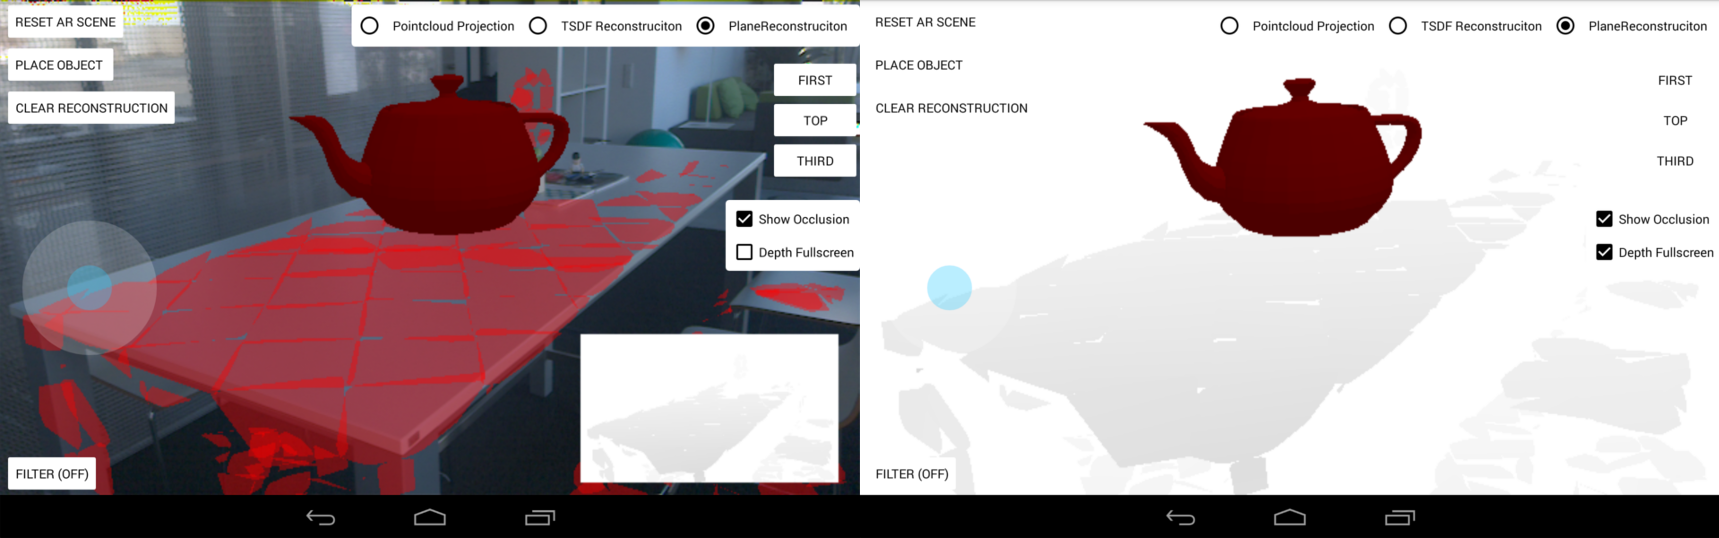
\includegraphics[width=1.0\textwidth]{content/images/implementation/plane-demo.png} 
  \caption{Planare Rekonstruktion Prototyp. Links optionale Projektion auf der Bildebene. Rechts das resultierende Tiefenbild.}
  \label{fig:plane-demo}
\end{figure}

Für die Berechnung mit Vektoren und Matrizen wurde wie auch im gesamten Projekt die OpenGL Mathematics Bibliothek (GLM)\footnote{OpenGL Mathematics - http://goo.gl/2oY83s (27.02.16)} verwendet. Sie bietet typische Primitiven mit entsprechenden Operationen für Berechnungen der linearen Algebra. Wie bereits beschrieben wird für die lineare Regression die Berechnung von Eigenvektoren mit ihren Eigenwerten benötigt. Diese Berechnung wird von GLM nicht unterstützt. Hier wurde die Eigen-Bibliothek\footnote{Eigen: template library for linear algebra - http://goo.gl/TsNOuW (27.02.16)} verwendet, die diese Operation für den Anwender anbietet. Abbildung \ref{fig:plane-demo} zeigt die Ergebnisse der Ebene Rekonstruktion Links und der daraus Resultierenden Tiefeninformation Rechts.




\subsubsection*{TSDF Rekonstruktion}

\citet{Klingensmith_2015_7924} erwähnen, dass ihr Verfahren Chisel zunächst als proprietäre Umsetzung im Project Tango Constructor\footnote{Project Tango Constructor - https://goo.gl/8HdTnY (27.02.16)}, Googles Demo Anwendung zur räumlichen Rekonstruktion, umgesetzt wurde. Zu Ihrer Publikation haben sie jedoch zusätzlich eine Open-Source ROS basiertes Modul zur Verfügung gestellt. Diese Bibliothek mit dem Namen OpenChisel\footnote{OpenChisel - Chisel chunked TSDF library - https://goo.gl/nla8hy (27.02.16)} wurde für den Prototypen auf Android NDK portiert. Dafür wurden einige Module des C++11 Standards, wie zum Beispiel \enquote{st::shared\_ptr}, die zum derzeitigen Kenntnisstand vom Android NDK nicht unterstützt werden, auf die Boost\footnote{Boost C++ Libraray - http://www.boost.org/ (27.02.16)} Implementationen abgeändert. Neben der Boost Bibliothek nutzt OpenChisel auch die Eigen Bibliothek für Primitiven und Berechnungen der linearen Algebra.\\

Als Eingabe benötigt OpenChisel neben der Kameraposition und Kameraeigenschaften entweder einer Pointcloud oder ein Tiefenbild. In der Proof of Concept Umsetzung war erkennbar, dass OpenChisel mit der Pointcloud von Project Tango deutlich schlechtere Ergebnisse lieferte, als die Implementation des Constructors von Google. Dadurch die Support Bibliothek von Google seit Februar 2016 eine performante Methode\footnote{TangoSupport\_upsampleImageNearestNeighbor - https://goo.gl/mchIie (27.02.16)} anbietet, um aus einer Punktewolke eine DepthMap mit einer Auflösung von \(320x180 \) zu generieren, wird nun ein Tiefenbild für OpenChisel verwendet. Die resultierenden Ergebnisse kommen dadurch der Constructor Implementation deutlich näher. Abbildung \ref{fig:chisel-demo} zeigt eine exemplarische Rekonstruktion eines Tiefenbildes links mit dem resultierenden Tiefenbild rechts.

\begin{figure}[h]
  \centering
	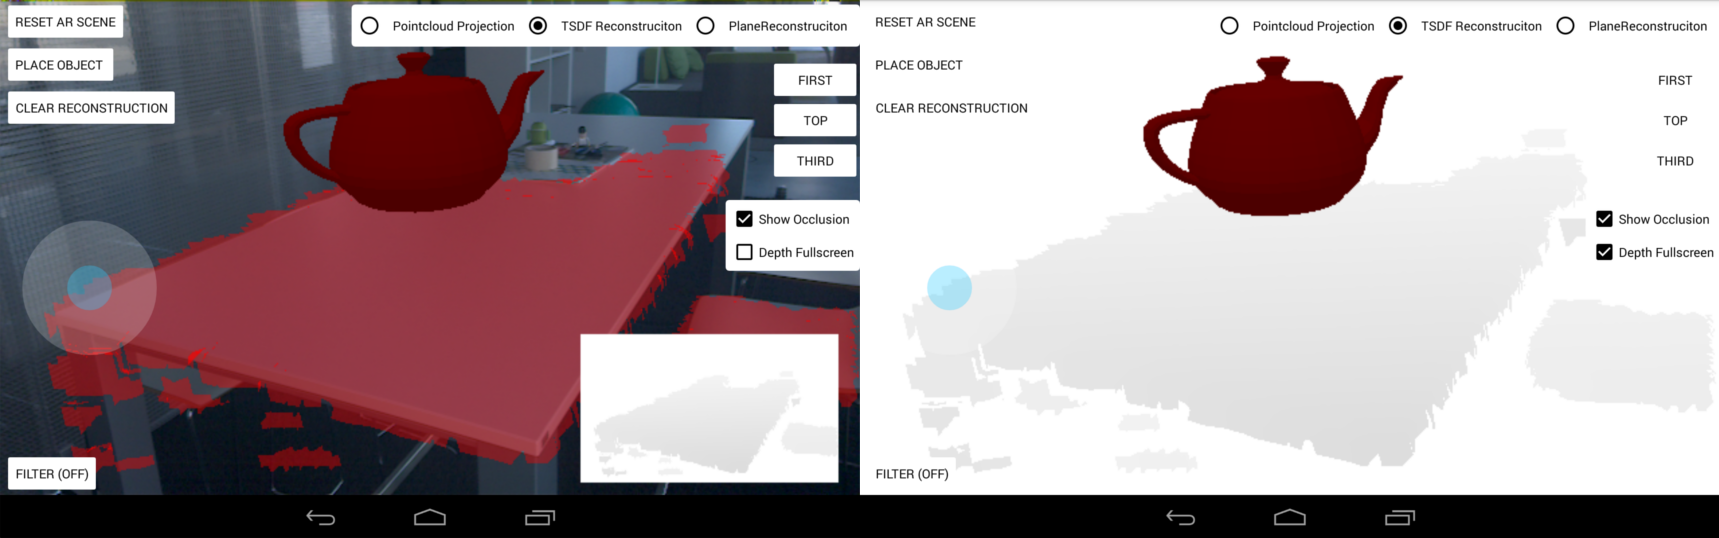
\includegraphics[width=1.0\textwidth]{content/images/implementation/chisel-demo.png} 
  \caption{OpenChisel Rekonstruktion Prototyp. Links optionale Projektion auf der Bildebene. Rechts das resultierende Tiefenbild.}
  \label{fig:chisel-demo}
\end{figure}


\subsubsection*{Guided Filter}

Für die Anwendung des Guided Filters wurde, wie bereits erwähnt, die Computer Vision Bibliothek OpenCV verwendet. Um diesen Filter mit OpenCV anwenden zu können mussten zuvor das RGB Bild und das Tiefenbild in das OpenCV Format gebracht werden. Dies war jedoch mit den Methoden \enquote{glReadPixels} und \enquote{glTexImage2D} für den aktuell selektierten Framebuffer und der OpenGL Textur problemlos möglich. Zwar sind die Speicherkonventionen von OpenGL und OpenCV, was die X und Y Achse angeht, genau vertauscht, jedoch ist das Filtern, welches daraus folgend gedreht stattfindet, für den Nutzer völlig intransparent und muss nicht weiter berücksichtigt werden.\\

Problematisch ist jedoch, dass das OpenGL Tiefenbild eine Farbtiefe von 16Bit nutzt und der OpenCV Guided Filter nur auf 8Bit Graustufen angewendet werden kann. Diese Transformation und die daraus resultierende Ungenauigkeit der Tiefe wurde jedoch zunächst in Kauf genommen, da erst einmal der Mechanismus als solches getestet werden soll. In der späteren Auswertung von Testszenarien muss diese Transformation berücksichtigt werden. \\

Diese Implementierung ermöglicht es, den Guided Filter dynamisch auf das aktuell generierte Tiefenbild mit dem aktuell aufgenommen RGB Bild als Leitbild anzuwenden. Außerdem lassen sich die Filter Parameter, dem Radius \(r\) und den Einflussfaktor \(\epsilon\) dynamisch variieren. Abbildung \ref{fig:filter-demo} zeigt das Tiefenbild der TSDF Rekonstruktion links, auf die rechts der Guided Filter mit dem aktuellen RGB Bild angewendet wurde. \\

\begin{figure}[h]
  \centering
	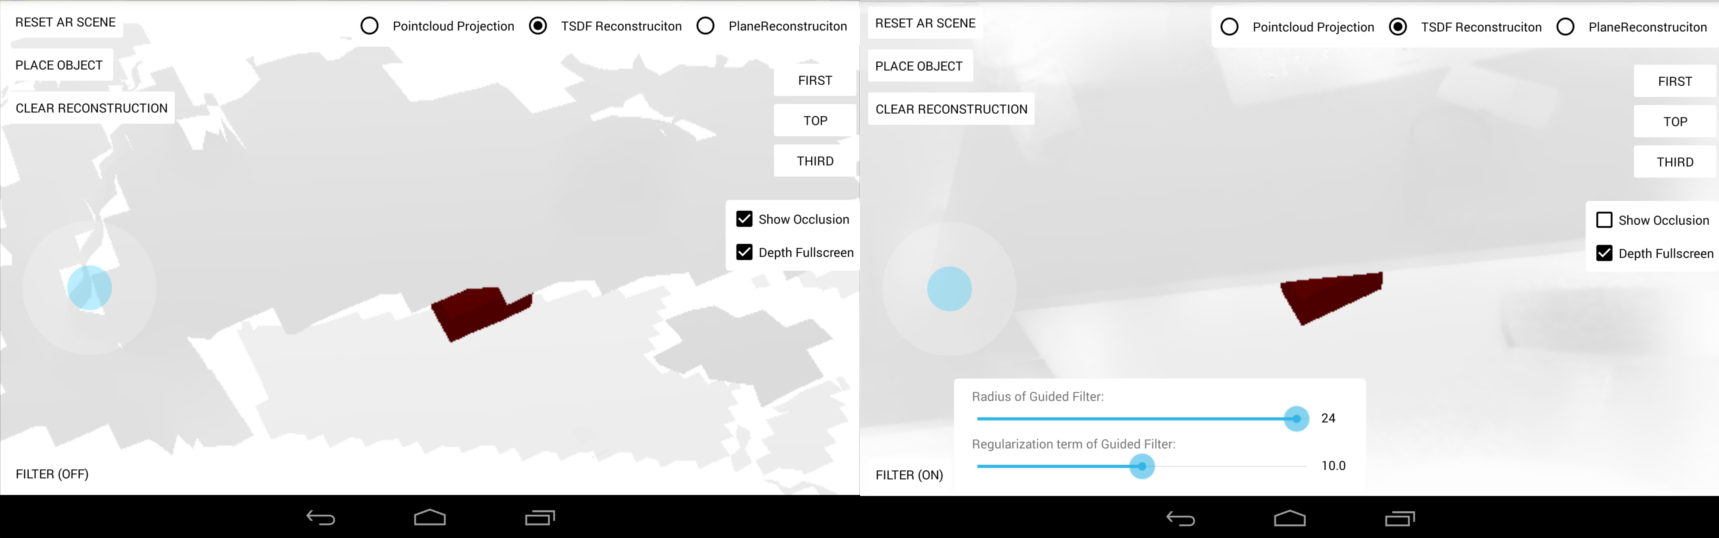
\includegraphics[width=1.0\textwidth]{content/images/implementation/filter-demo.png} 
  \caption{Anwendung des Guided Filters auf eine TSDF Rekonstruktion. Links vor und rechts nach der Anwendung.}
  \label{fig:filter-demo}
\end{figure}





% Evaluation
\chapter{Evaluation}

In diesem Kapitel sollen die beschriebenen und prototypisch implementierten Verfahren zur Überlagerung gegenübergestellt werden, um anhand eines direkten Vergleichs eine objektive Aussage über die Qualität der Ergebnisse treffen zu können. Hierzu wird im ersten Teil das Vorgehen zum Testen vorgestellt, welches darauf folgend mit allen Verfahren umgesetzt wird. Hiernach werden die daraus resultierenden Ergebnisse gegenübergestellt.

\section{Statische Testszenen}

Zum Vergleich der Verfahren wurden zwei statische Szenen gewählt, in denen das Project Tango Gerät nicht bewegt wird und für alle Kandidaten den selben Inhalt bietet. Diese Wahl wurde getroffen, um eine zuverlässige und reproduzierbare Informationsquelle für das Gerät zu schaffen. Denn die Reproduktion eines bewegten und dynamischen Szenarios ist für alle zu vergleichenden Verfahren nur sehr schwer möglich. \\

Eine mögliche Idee für ein dynamisches Testszenario war es, alle sensorischen Informationen der Hardware einmal aufzunehmen und eine reproduzierbare simulierte Umgebung dieser Daten zu schaffen. Technologien wie das Robot Operating System (ROS) würden dies ermöglichen, jedoch übersteigt der Aufwand den zeitlichen Rahmen dieser Arbeit. Auch wenn die Firma Bosch eine exemplarische Implementation\footnote{Tango Output to Rosbag Files - https://goo.gl/hhnciZ} für die Aufnahme aller Daten in ROS demonstriert, sind die implementierten Verfahren zu sehr in den API Zyklen der Project Tango Schnittstelle involviert, um diese in kurzer Zeit auf eine Desktop Umgebung zu portieren.\\

Die erste gewählte Szene, welche in Abbildung \ref{fig:static-scene} links zu sehen ist, beinhaltet einen Hocker, in Form eines einfachen  Würfels, und einen Sitzball. Der Sitzball wurde gewählt, um auch runde Formen zur Tiefenaufnahme zu testen. Das Project Tango Gerät ist etwas höher in einem Stativ plaziert. Das virtuelle Objekt wird, wie in Abbildung \ref{fig:static-scene} rechts, zwischen die beiden realen Objekte plaziert, sodass es von beiden Seiten durch die realen Objekte überdeckt wird. \\

\begin{figure}[h]
  \centering
	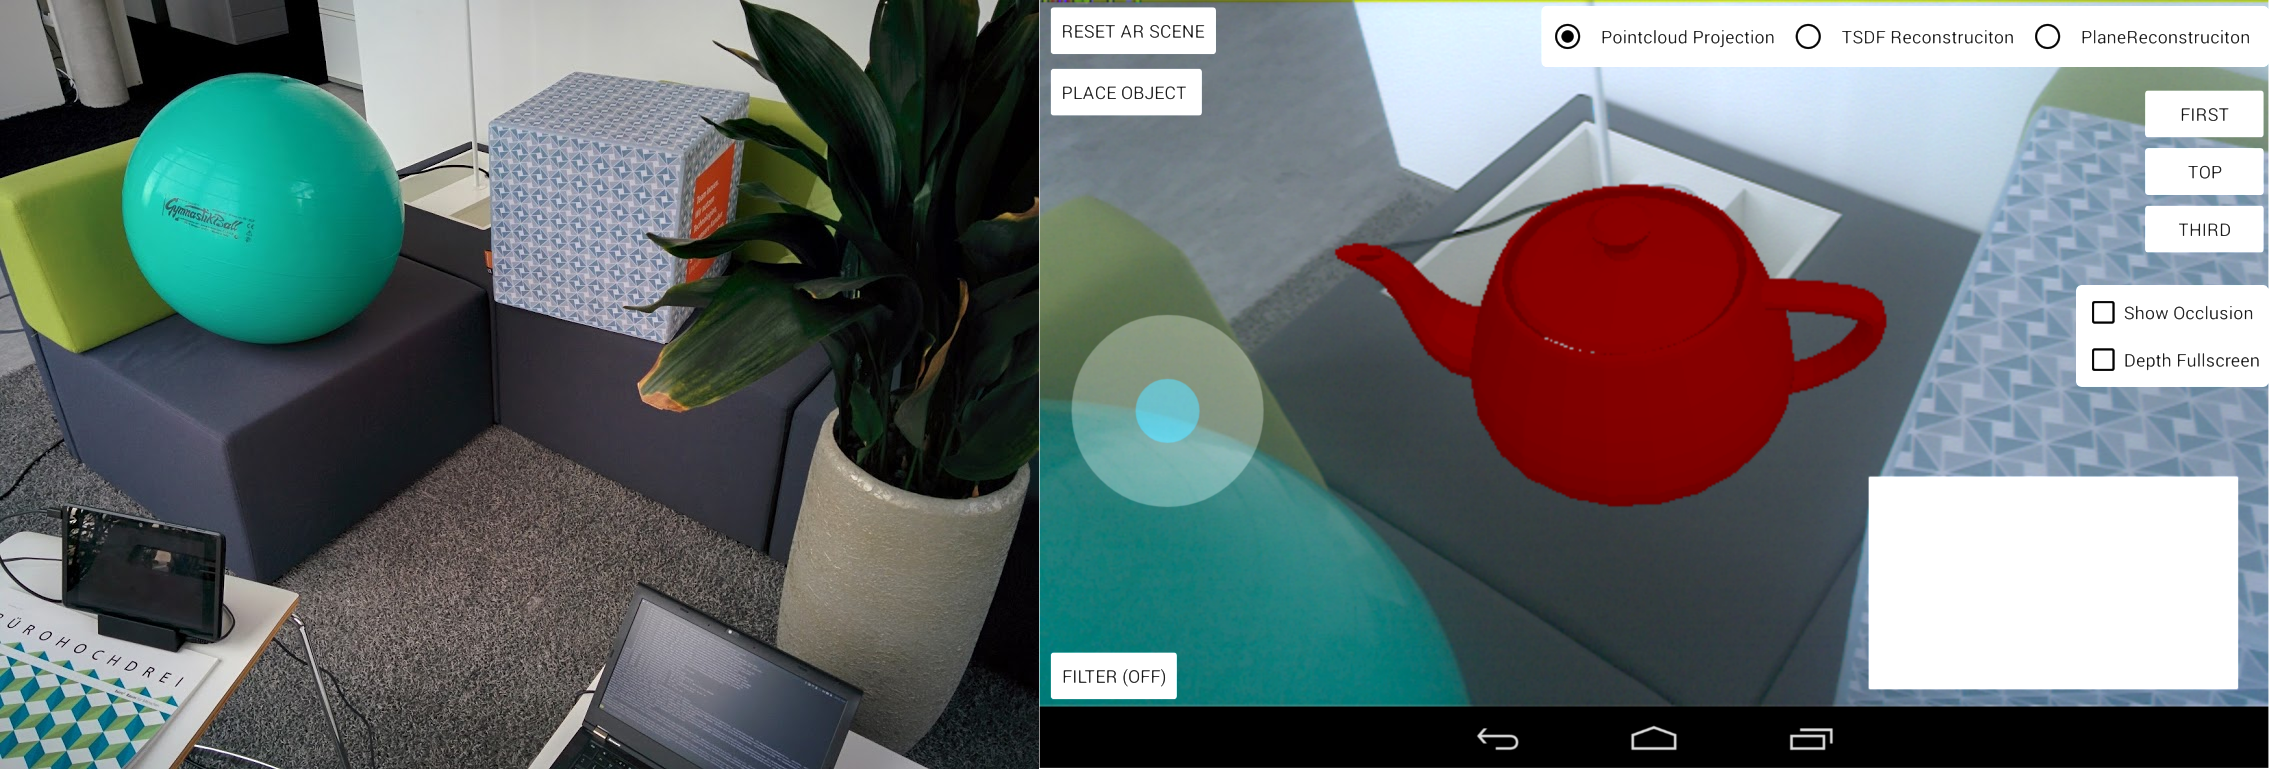
\includegraphics[width=1.0\textwidth]{content/images/evaluation/static-scene.png} 
  \caption{Links: Erste statische Szene mit einem Hocker und einem Sitzball. Rechts: Platzierung des virtuellen Objekts. }
  \label{fig:static-scene}
\end{figure}

Die zweite gewählte Szene, welche in Abbildung \ref{fig:plant-scene} links zu sehen ist, soll als Herausforderung die Überdeckung von komplexeren Strukturen testen. Sie besteht daher aus einer Pflanze, die sich, wie rechts im Bild zu sehen, vor dem virtuellen Objekt befindet. Auch hier befindet sich das Project Tango Gerät in einem Stativ.

\begin{figure}[h]
  \centering
	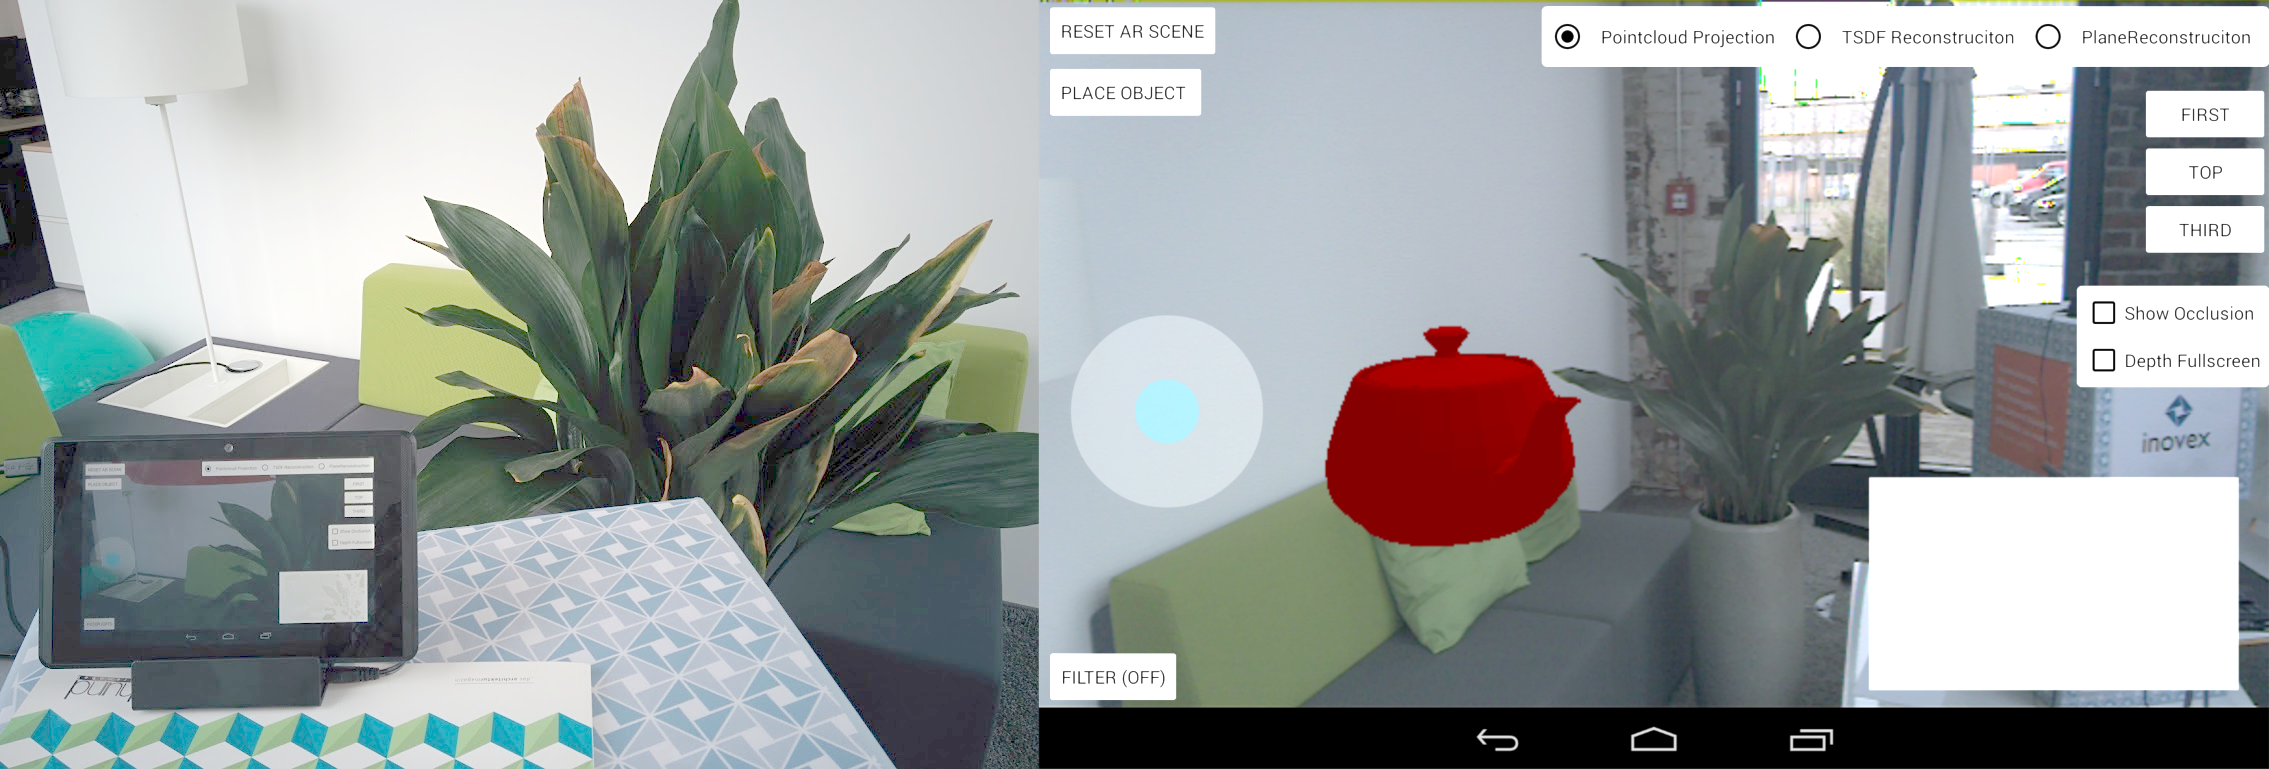
\includegraphics[width=1.0\textwidth]{content/images/evaluation/plant-scene.png} 
  \caption{Links: Zweite statische Szene mit einer Pflanze im Vordergrund. Rechts: Platzierung des virtuellen Objekts hinter der Pflanze. }
  \label{fig:plant-scene}
\end{figure}

Für beide Szenen sollen alle Kombinationen der Verfahren getestet werden. Somit ergeben sich sechs verschiedene Kombinationen, in denen die Pointcloud Projektion, die TSDF Rekonstruktion und die Ebenen Rekonstruktion jeweils mit und ohne dem Guided Filter getestet werden. Für alle Kombinationen soll ein gerendertes Bild und ein Tiefenbild mit dem virtuellen Objekt festgehalten werden. Zur Auswertung werden die jeweils gerenderten Ergebnisbilder mit einem manuell zugeschnittenem Ergebnisbild verglichen. Hierfür wird die Summe der absoluten Bilddifferenz wie in Gleichung \ref{eq:diff} bestimmt.

\begin{equation} \label{eq:diff}
d = \sum_i |p_i-q_i|
\end{equation}

\section{Durchführung der Tests}

\begin{figure}[h]
  \centering
	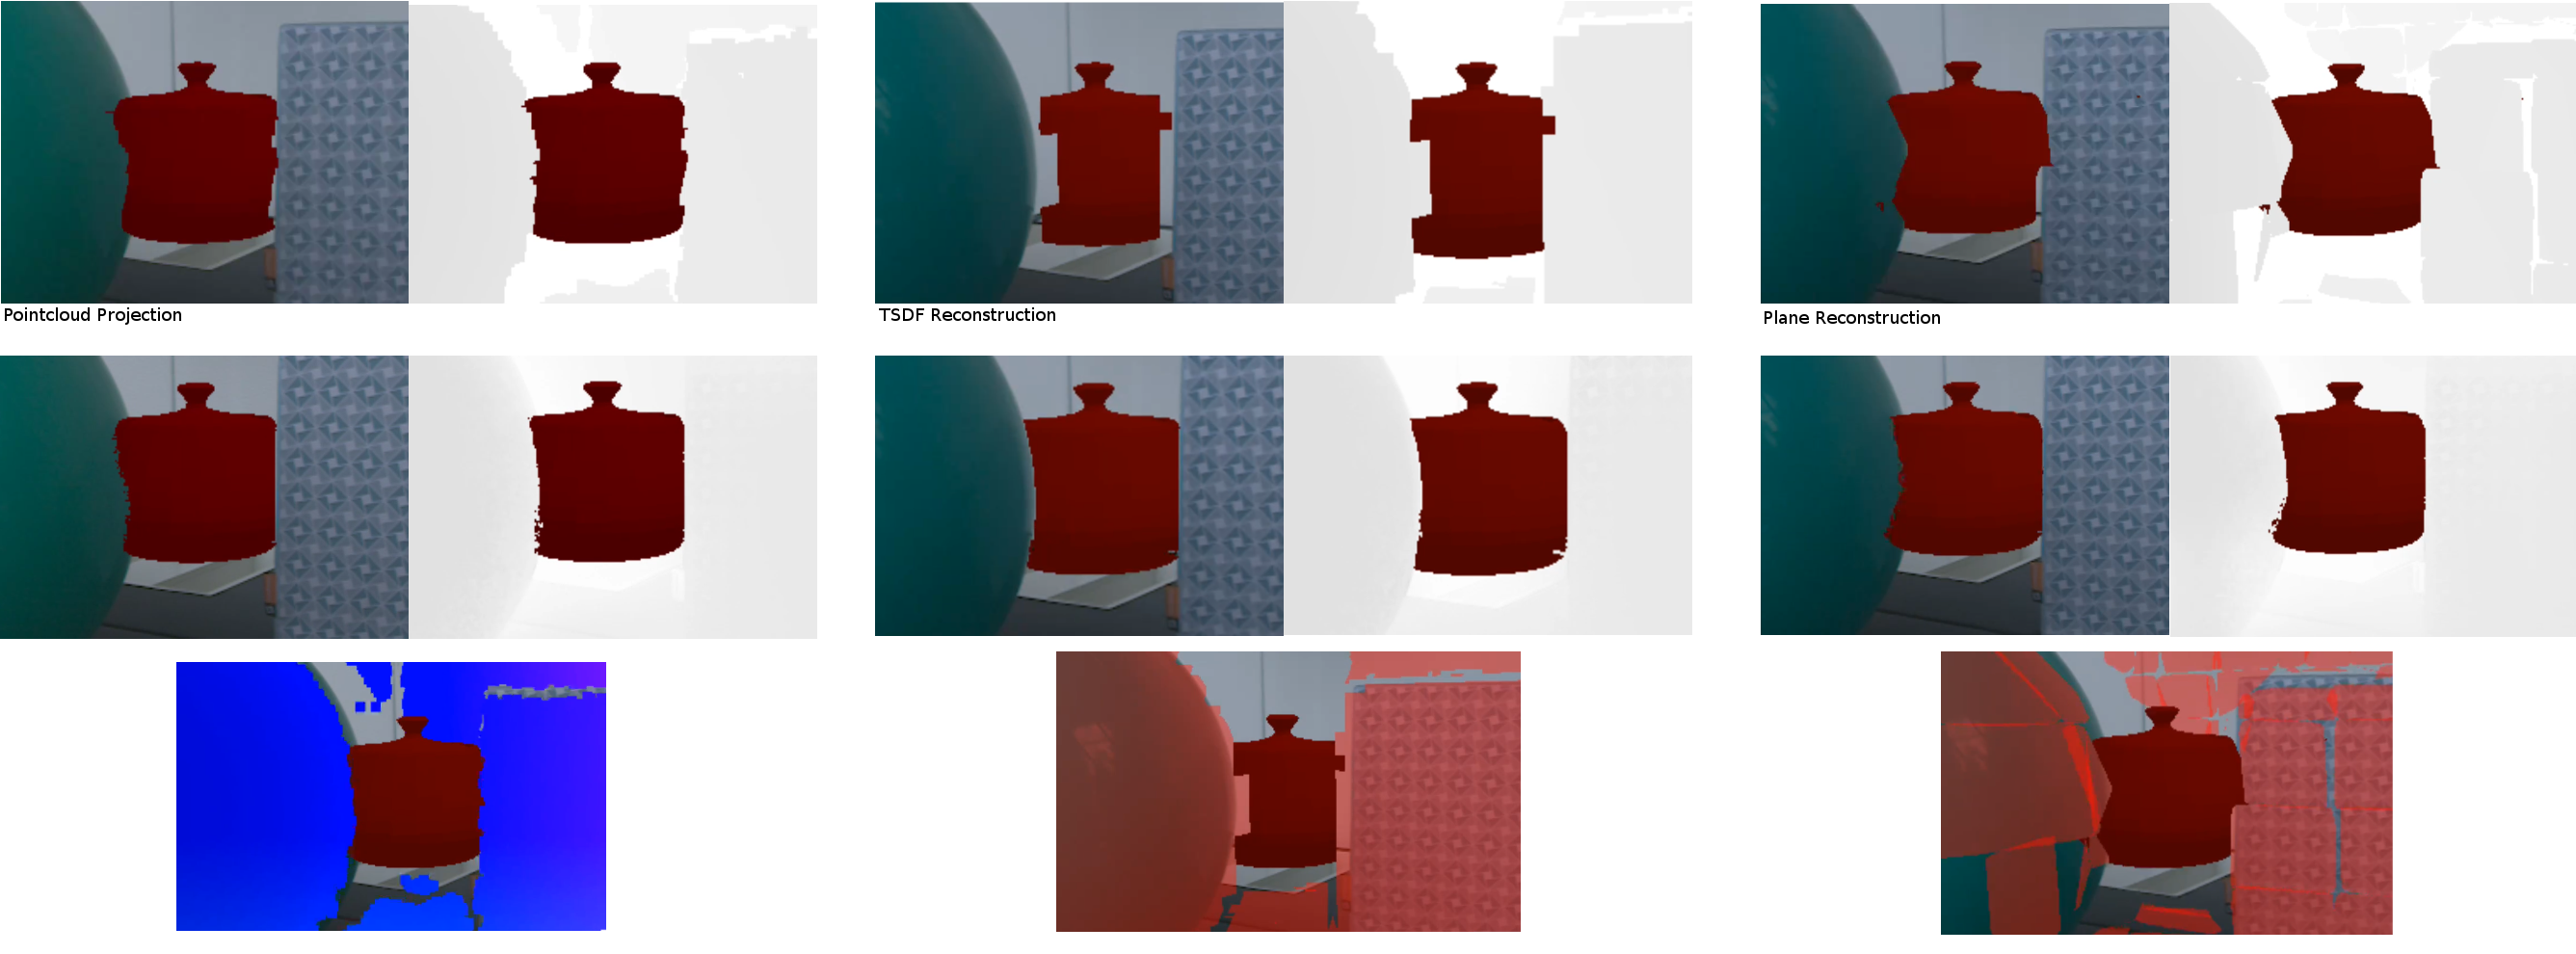
\includegraphics[width=1.0\textwidth]{content/images/evaluation/static_occlusion.png} 
  \caption{}
  \label{fig:static_occlusion}
\end{figure}

\begin{figure}[h]
  \centering
	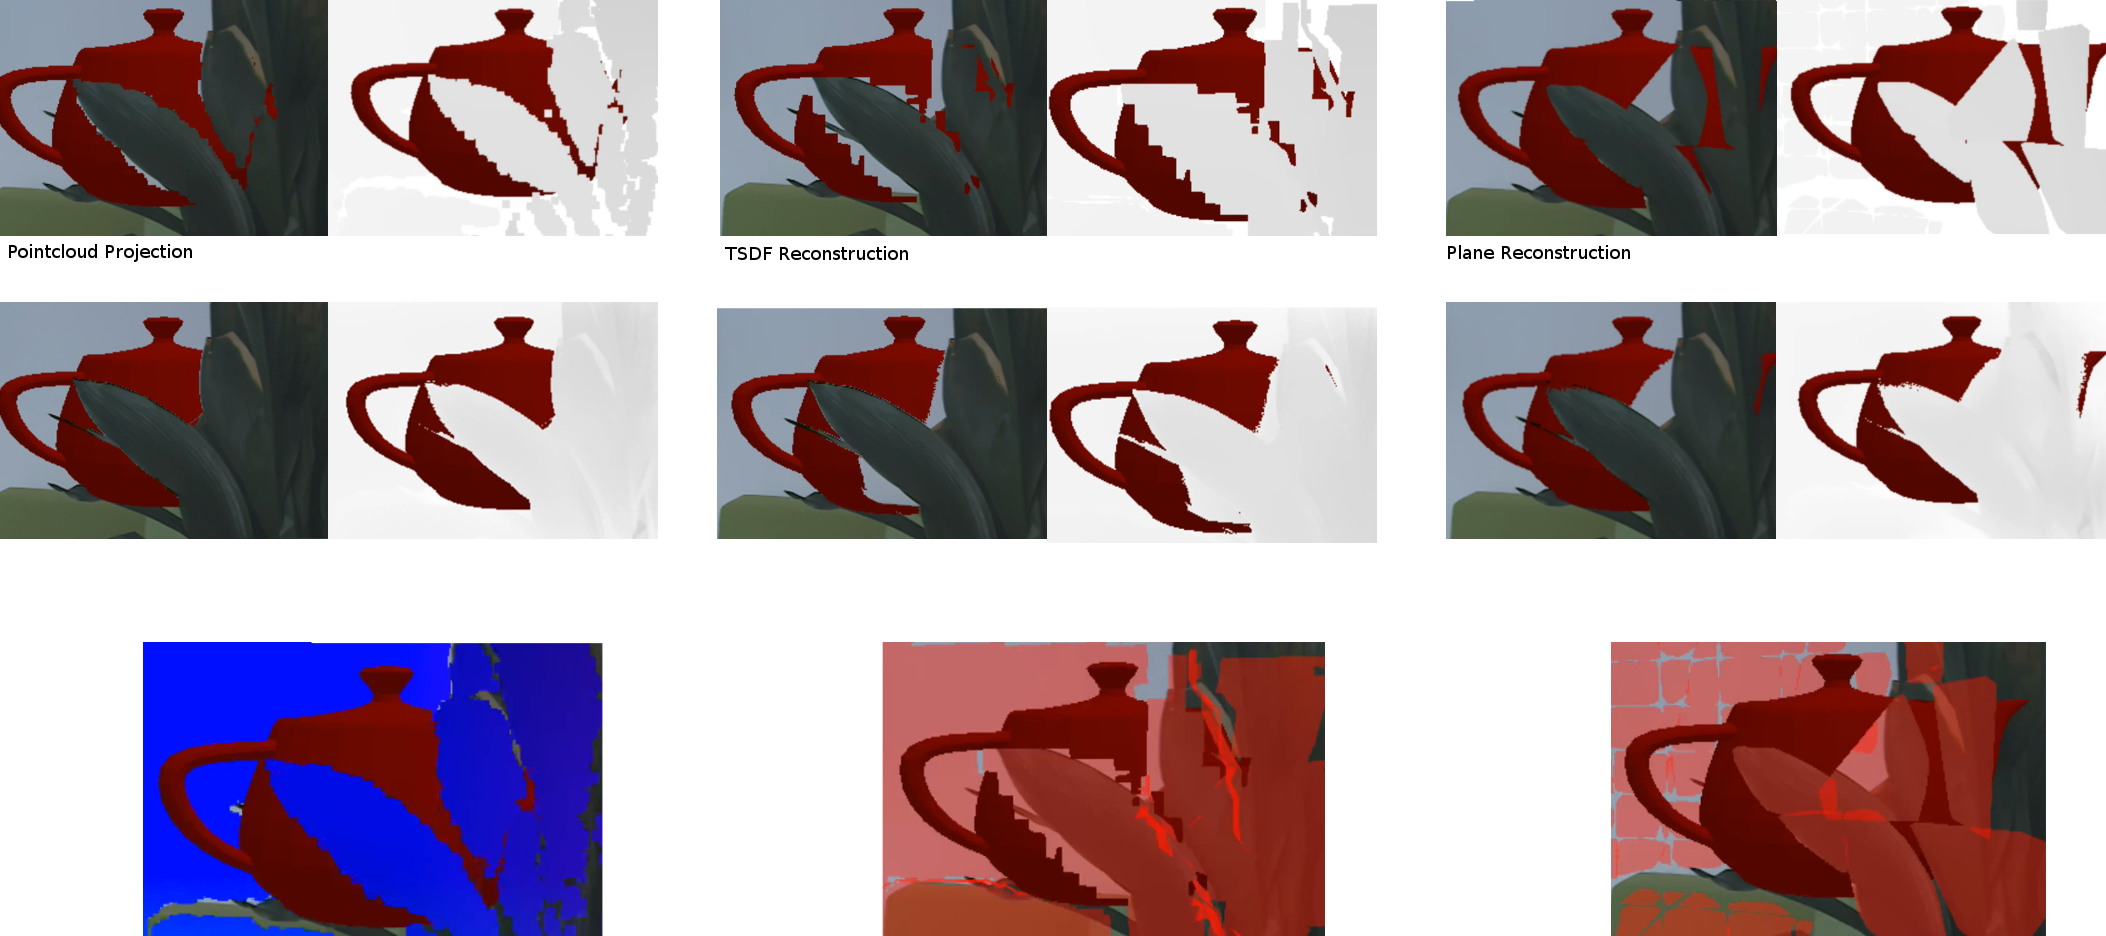
\includegraphics[width=1.0\textwidth]{content/images/evaluation/plant_occlusion.png} 
  \caption{}
  \label{fig:plant_occlusion}
\end{figure}

\section{Vergleich der Ergebnisse}

\begin{figure}[h]
  \centering
	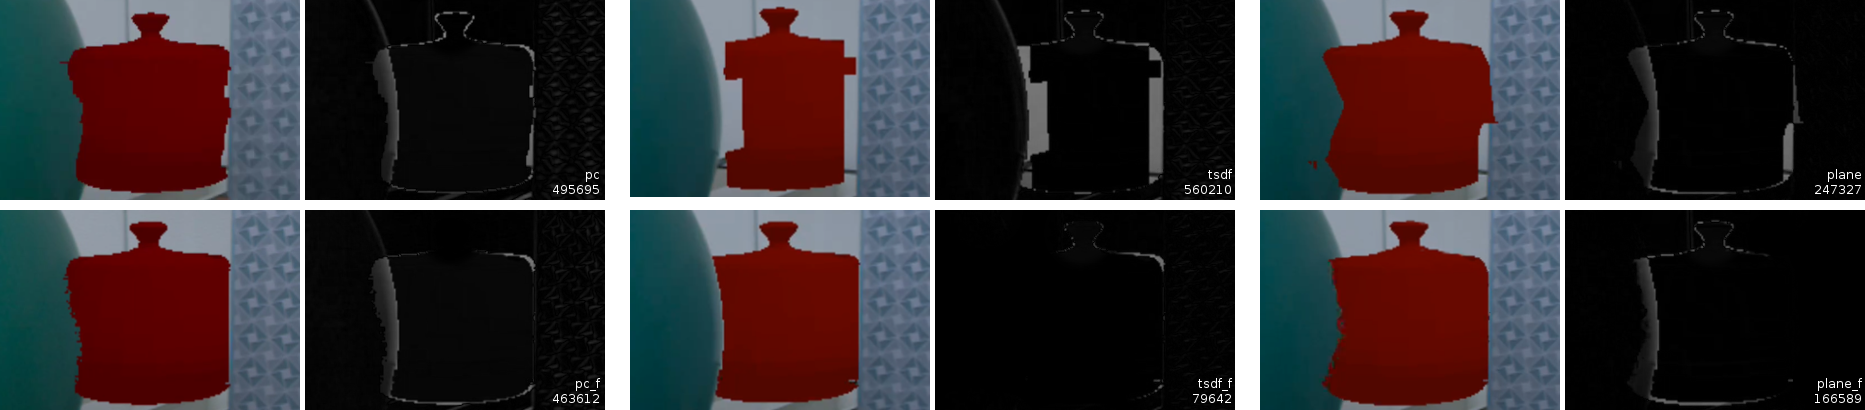
\includegraphics[width=1.0\textwidth]{content/images/evaluation/static_occlusion_results.png} 
  \caption{}
  \label{fig:static_occlusion_results}
\end{figure}

\begin{figure}[h]
  \centering
	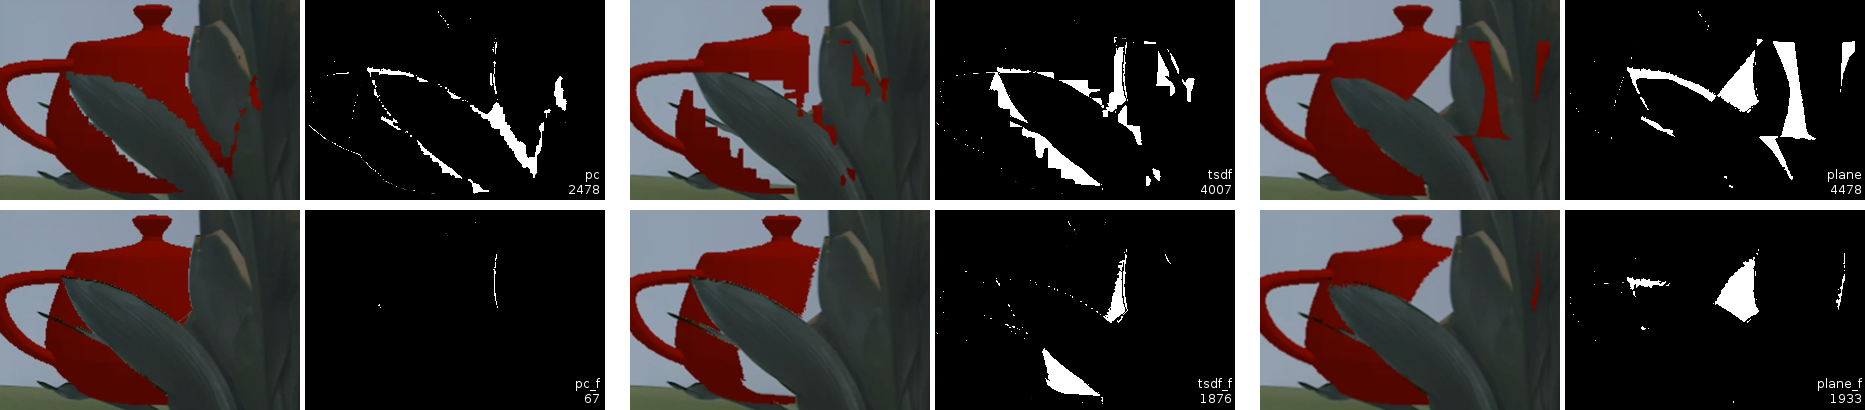
\includegraphics[width=1.0\textwidth]{content/images/evaluation/plant_occlusion_results.png} 
  \caption{}
  \label{fig:plant_occlusion_results}
\end{figure}

% Fazit
\chapter{Fazit}

* Light-Field Cameras als Kombination für AR!!

\appendix
\listoffigures
\lstlistoflistings  

\chapter{Ergebnisaufnahmen}
\begin{sidewaysfigure}[h]
  \centering
	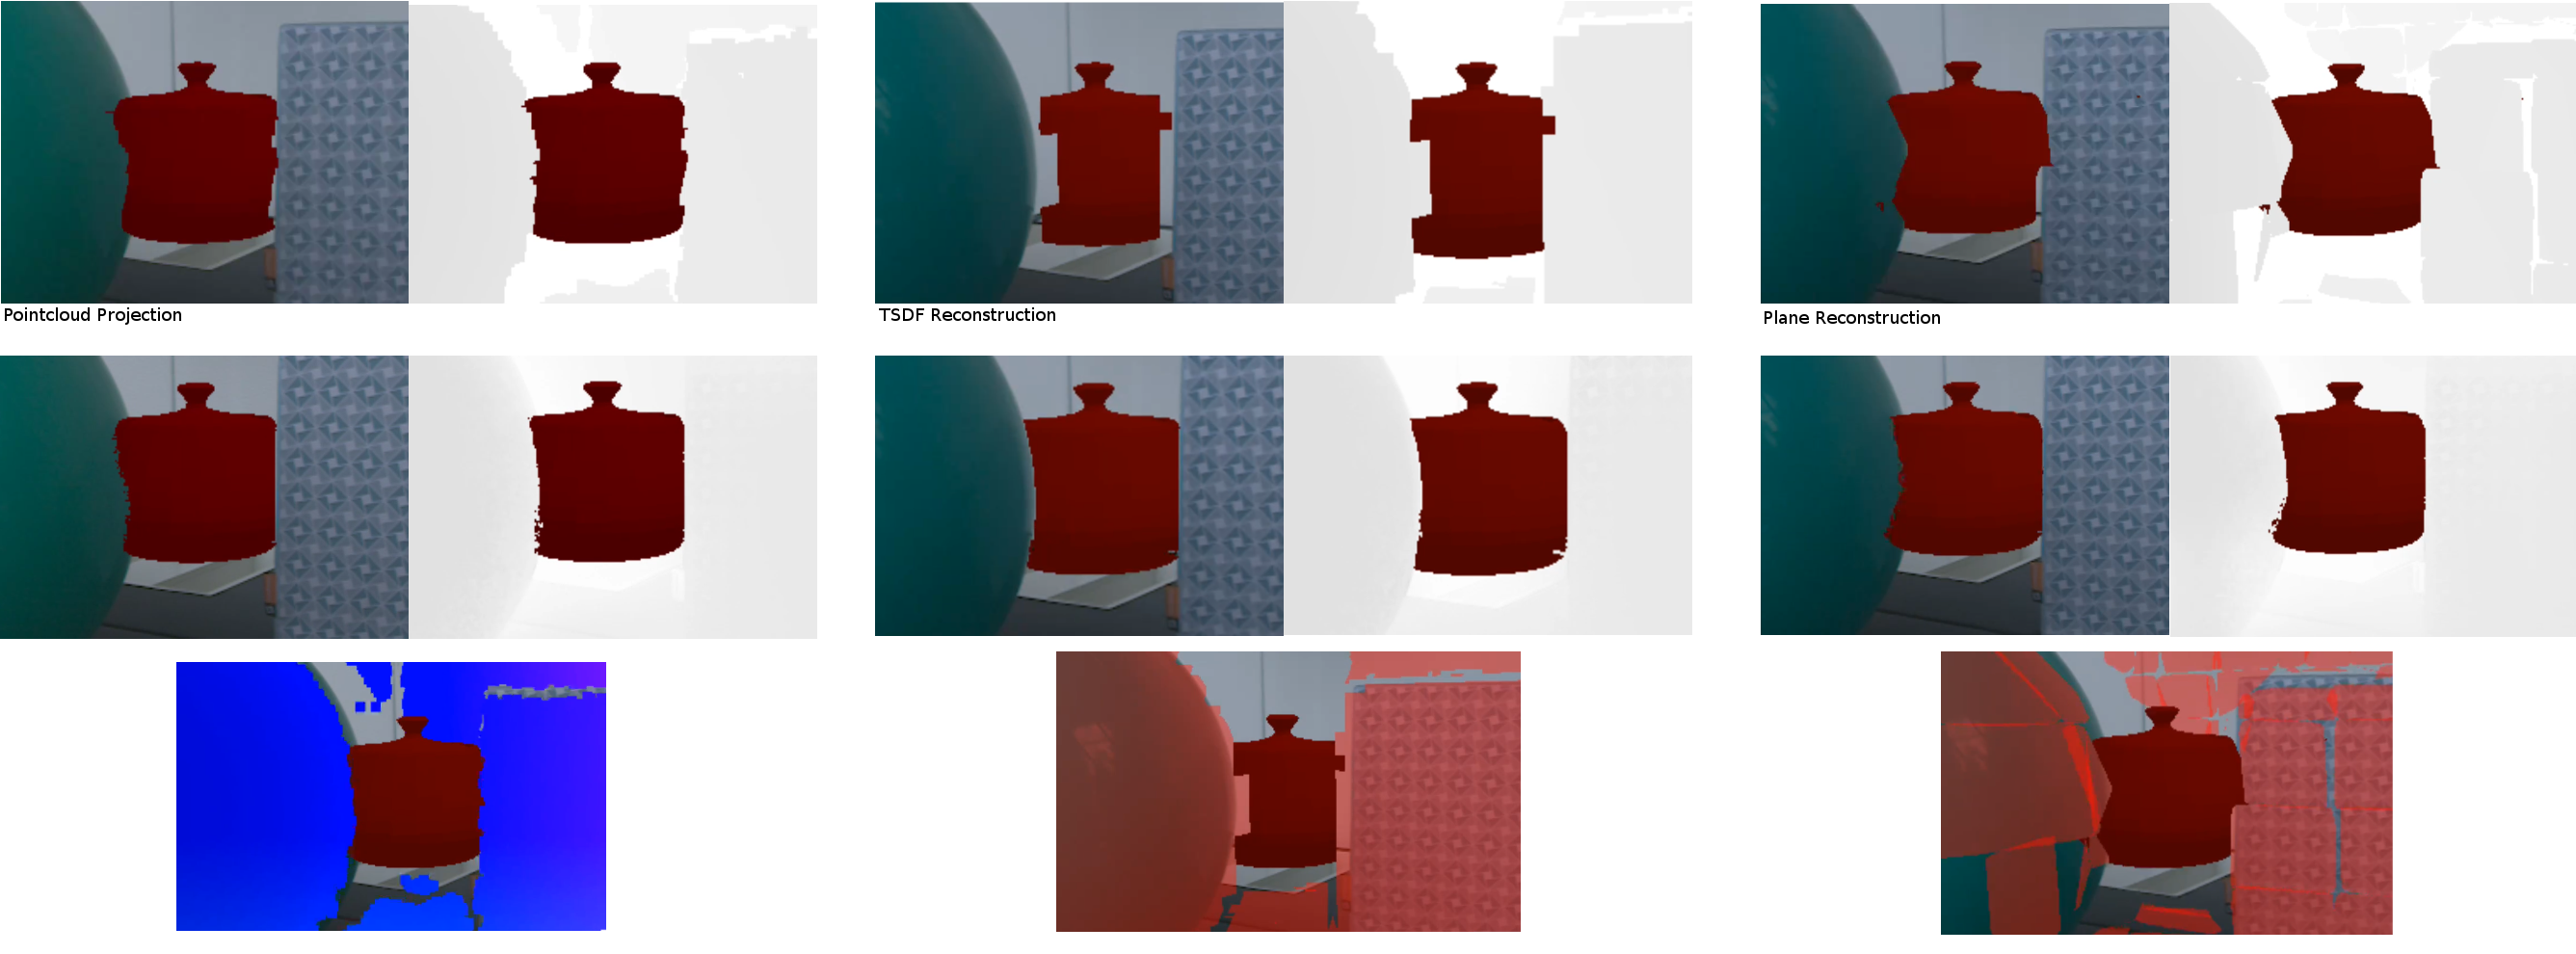
\includegraphics[width=1.0\textwidth]{content/images/evaluation/static_occlusion.png} 
  \caption{Ergebnisaufnahmen aus der ersten statischen Szene}
  \label{fig:static_occlusion}
\end{sidewaysfigure}

\begin{sidewaysfigure}[h]
  \centering
	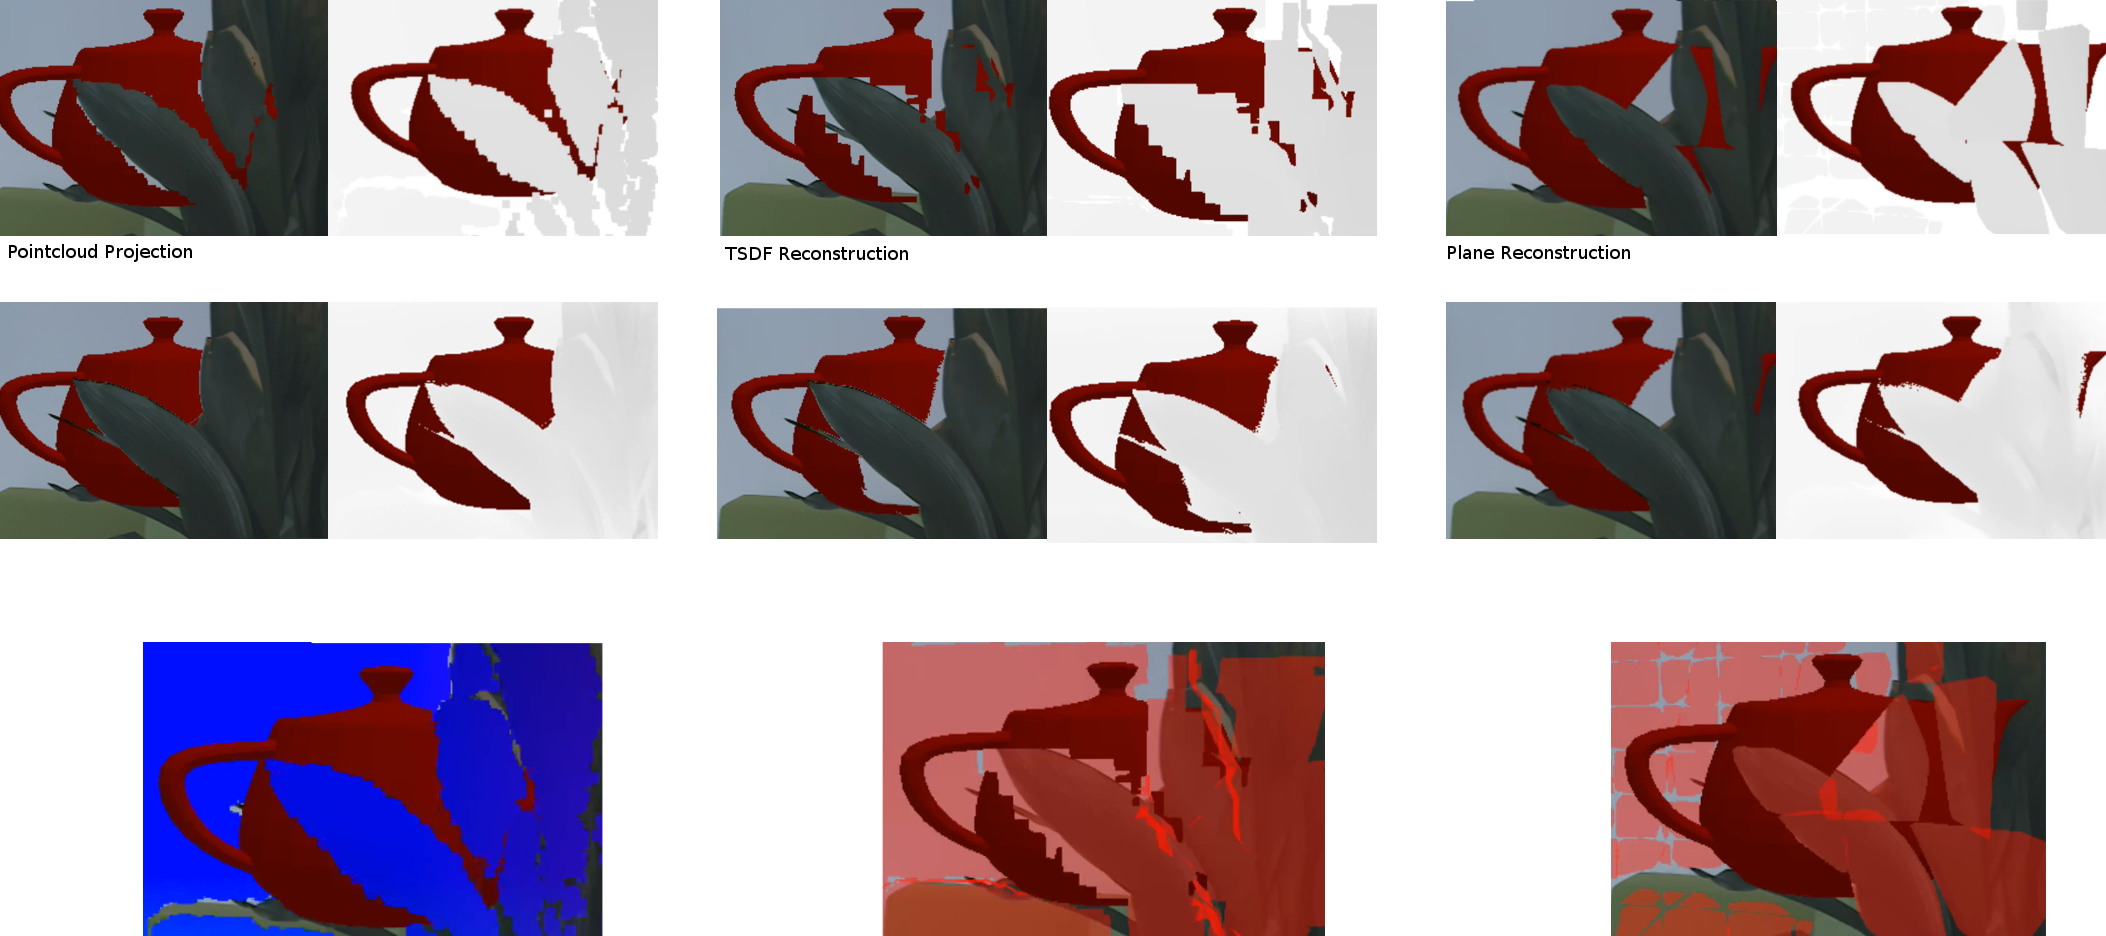
\includegraphics[width=1.0\textwidth]{content/images/evaluation/plant_occlusion.png} 
  \caption{Ergebnisaufnahmen aus der zweiten statischen Szene}
  \label{fig:plant_occlusion}
\end{sidewaysfigure}

\begin{sidewaysfigure}[h]
  \centering
	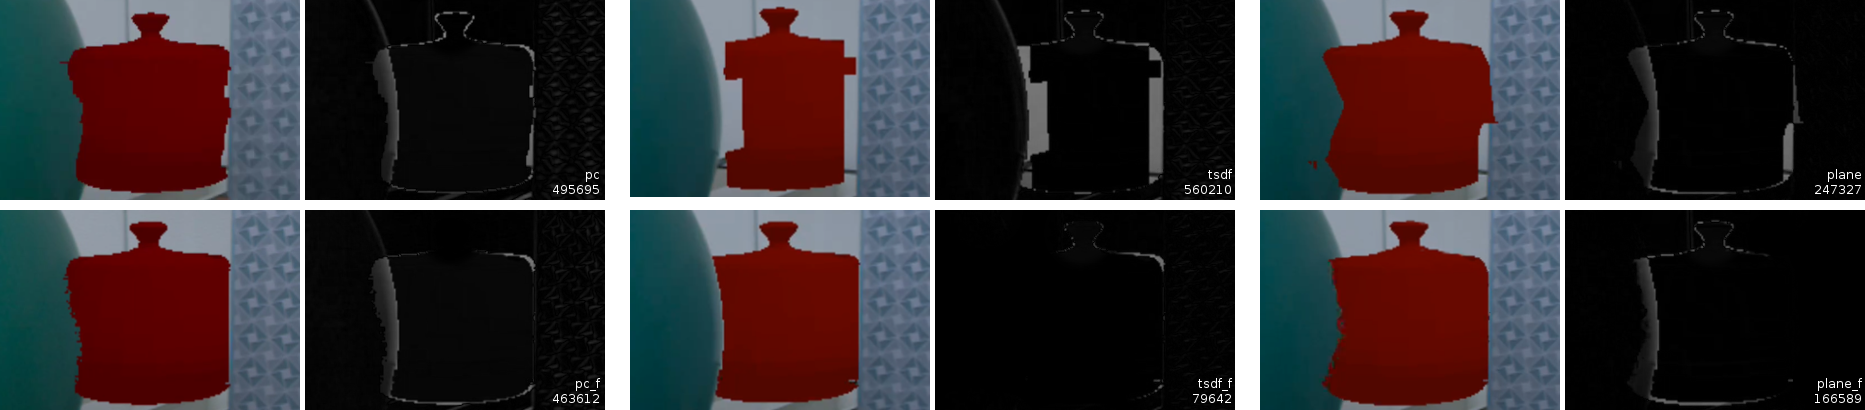
\includegraphics[width=1.0\textwidth]{content/images/evaluation/static_occlusion_results.png} 
	
\includegraphics[width=1.0\textwidth]{content/images/evaluation/spacer.png} 
	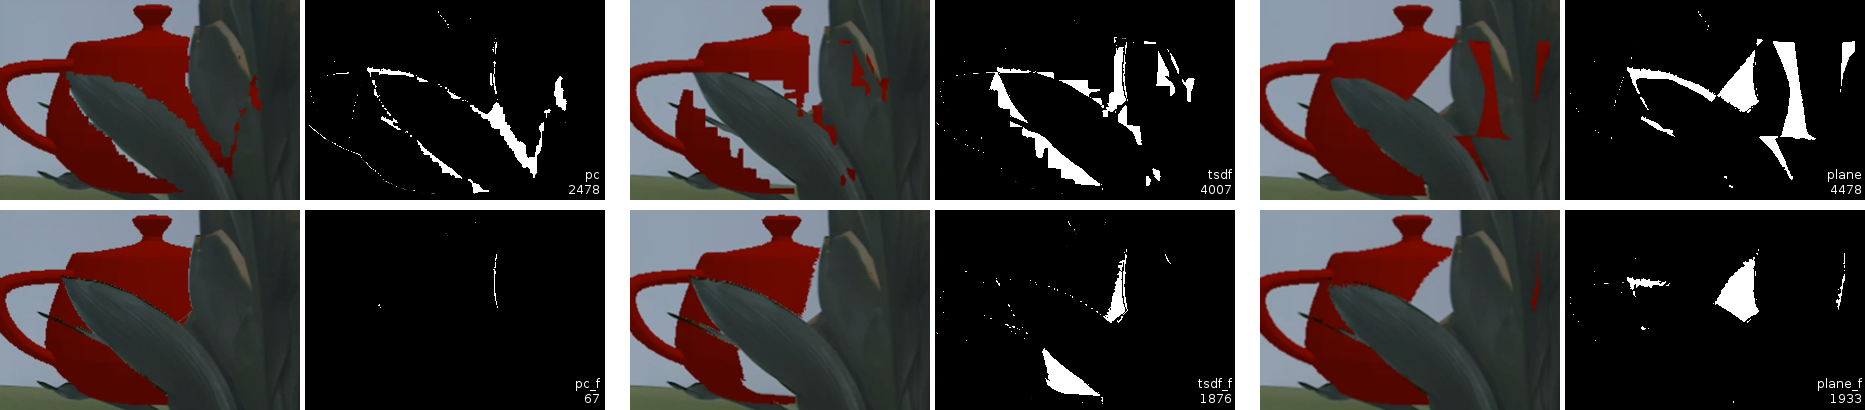
\includegraphics[width=1.0\textwidth]{content/images/evaluation/plant_occlusion_results.png} 
  \caption{Differenzbilder der Verfahren in ersten (oben) und zweiten Szene (unten)}
  \label{fig:static_occlusion_results}
\end{sidewaysfigure}


\addcontentsline{toc}{chapter}{Bibliography}

\bibliography{main}
\bibliographystyle{natdin} 

\end{document}

